\documentclass[10pt,twocolumn,letterpaper]{article}

\usepackage{./ICCV2023/iccv}
\usepackage{times}
\usepackage{epsfig}
\usepackage{graphicx}
\usepackage{amsmath}
\usepackage{amssymb}

\usepackage{graphicx}
\usepackage{amsmath}
\usepackage{amssymb}
\usepackage{booktabs}

\usepackage{threeparttable}
\usepackage[vlined, ruled, linesnumbered]{algorithm2e}
\usepackage{multirow}
\usepackage{booktabs}
\usepackage{bbm}
\usepackage{pifont}
\usepackage{enumitem}

\usepackage{eucal,nicefrac}
\usepackage{subcaption}
\usepackage{gensymb}




\usepackage[margin=4pt,font=footnotesize,labelfont=bf,labelsep=endash,tableposition=top]{caption}


\usepackage[pagebackref=true,breaklinks=true,letterpaper=true,colorlinks,bookmarks=false]{hyperref}



\usepackage[capitalize]{cleveref}
\crefname{section}{Sec.}{Secs.}
\Crefname{section}{Section}{Sections}
\Crefname{table}{Table}{Tables}
\crefname{table}{Table}{Tables}

\iccvfinalcopy %

\def\iccvPaperID{5522} %
\def\httilde{\mbox{\tt\raisebox{-.5ex}{\symbol{126}}}}

\ificcvfinal\pagestyle{empty}\fi

\begin{document}

\title{Metric3D: Towards Zero-shot Metric 3D Prediction from A Single Image}


\def\SP{~~}

\author{
Wei Yin$^{1 \ast}$,
\SP
Chi Zhang$^2$\thanks{Equal contributions.}, 
\SP 
Hao Chen$^3$\thanks{Corresponding author.},
\SP
Zhipeng Cai$^4$,
\SP 
Gang Yu$^2$,
\SP 
Kaixuan Wang$^1$, \\
\SP 
Xiaozhi Chen$^1$,
\SP 
Chunhua Shen$^3$
\\[0.1325cm]
$ ^1$ DJI Technology
\SP ~~~
$ ^2 $ Tencent
\SP ~~~
$ ^3$ Zhejiang University
\SP ~~~
$ ^4$ Intel Labs
\\
{e-mail: $\tt\small ^1 \{yvan.yin, halfbullet.wang, xiaozhi.chen\}@dji.com;$ }\\
$ \tt\small^2\{johnczhang, skicyyu\}@tencent.com;$ \\
$ \tt\small ^3 haochen.cad@zju.edu.cn, chunhua@me.com;$ 
$\tt\small ^4 zhipeng.cai@intel.com$ 
}




\makeatletter
\let\@oldmaketitle\@maketitle%
\renewcommand{\@maketitle}{\@oldmaketitle%
 \centering
    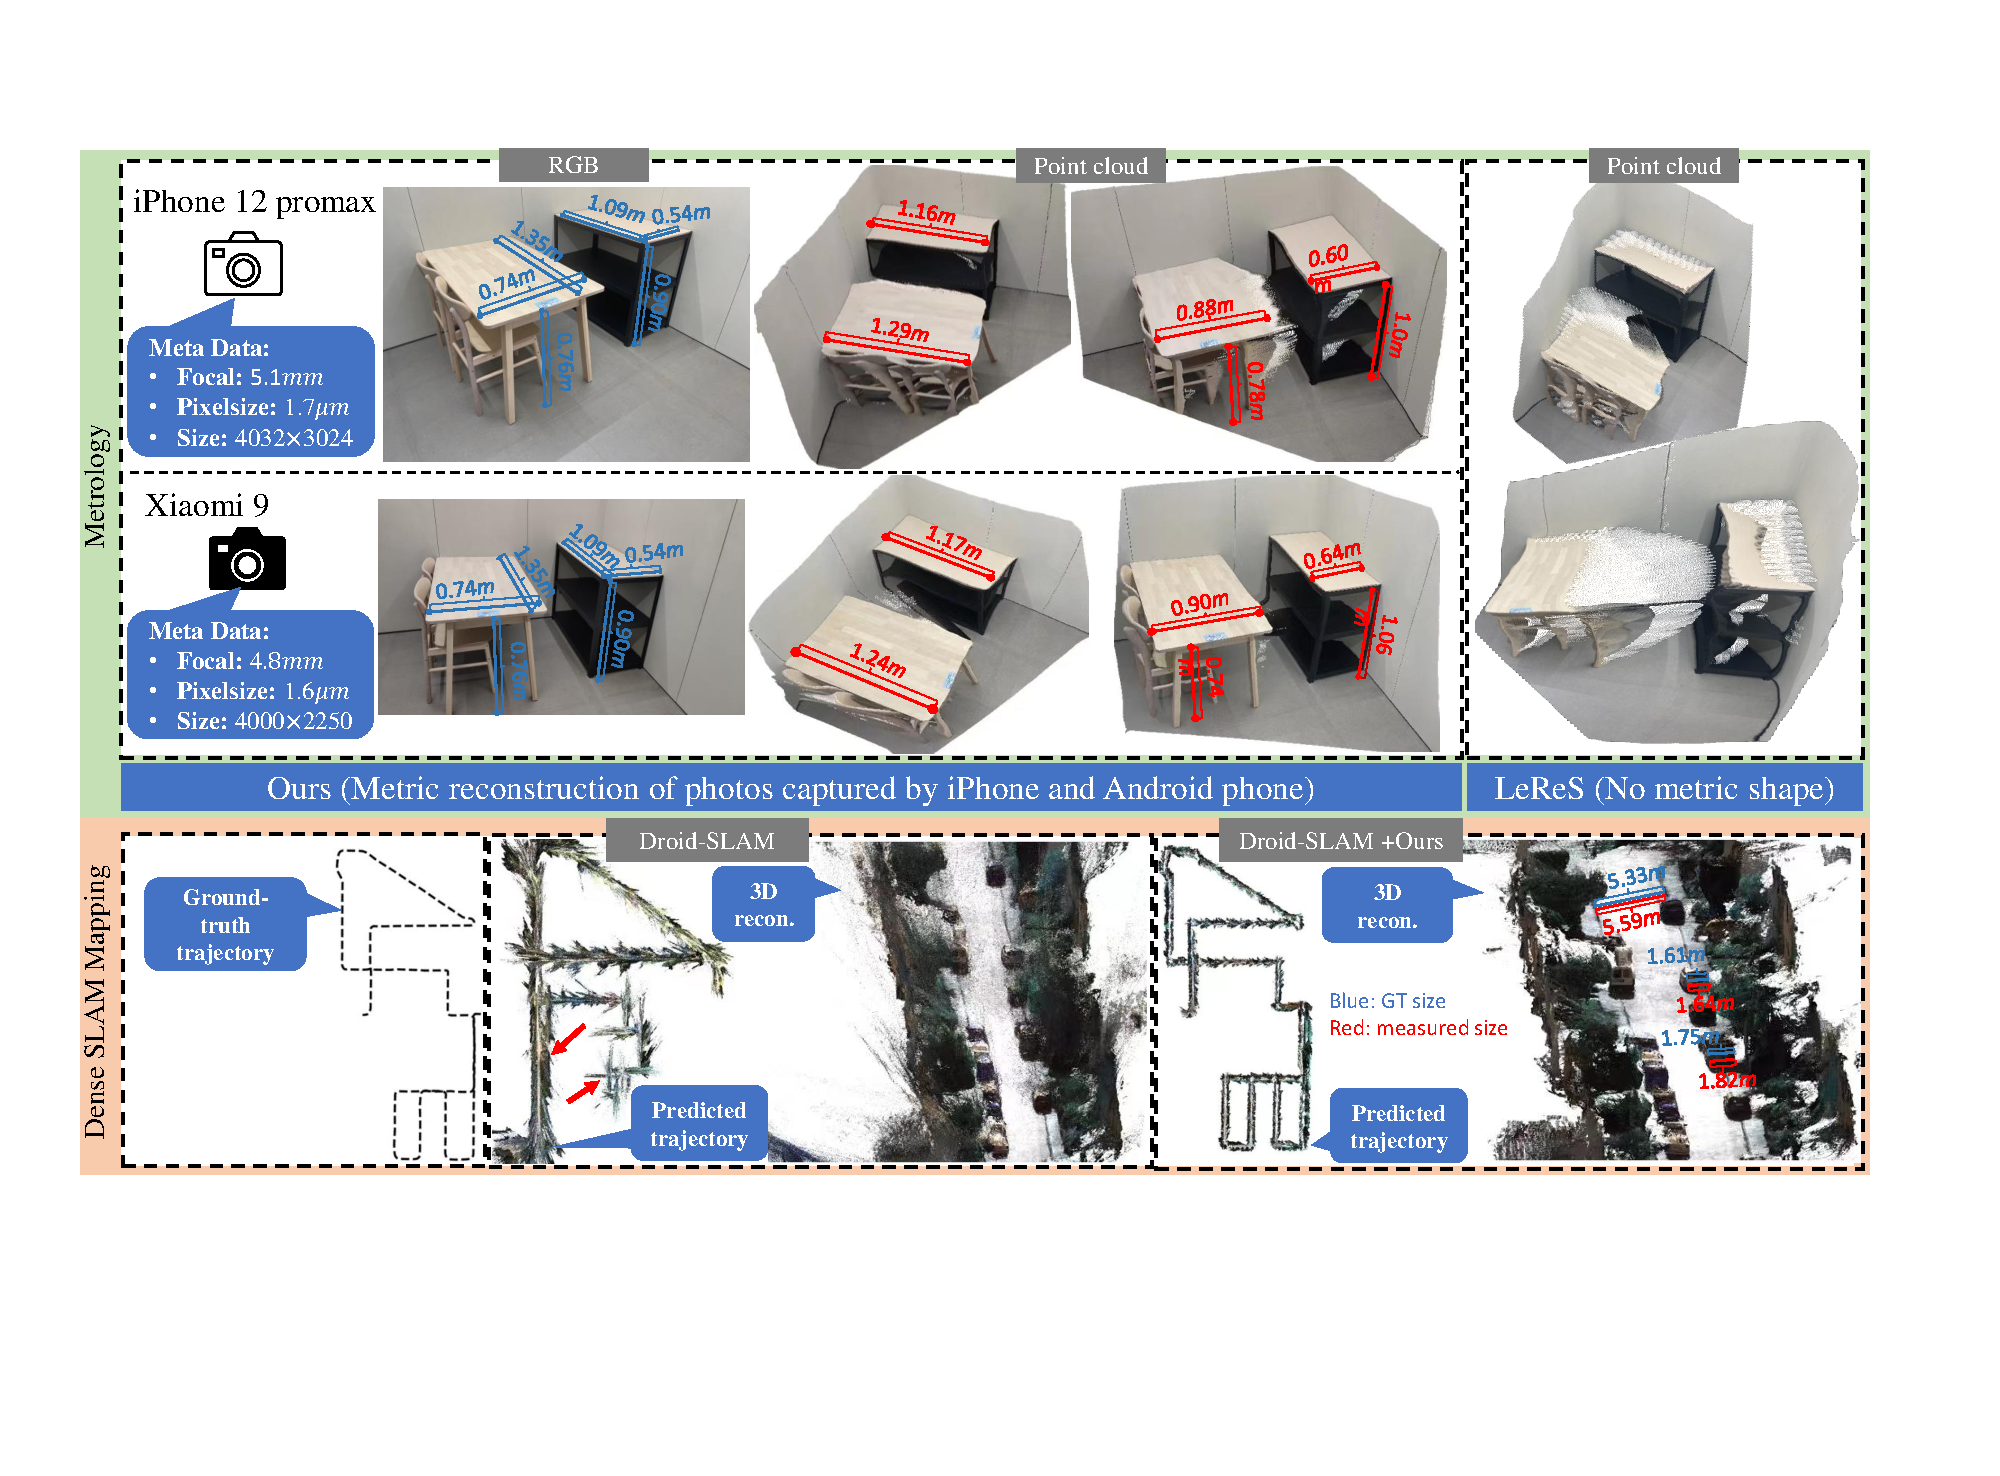
\includegraphics[width=0.95\textwidth]{./files/front_img.pdf}
     \captionof{figure}{\textbf{
     Illustration 
     and applications of our metric 3D reconstruction
     method}.
     Top (metrology):  we use two phones (iPhone 12 and an Android phone) to capture the scene and measure the size of tables. With the photos' metadata, we perform 3D metric reconstruction and then measure tables' sizes (marked in red), which are very close to the ground truth (marked in blue). In contrast, the recent method LeReS~\cite{leres} performs much worse and is unable to predict metric 3D by design.
     Bottom  (dense SLAM mapping): existing SOTA mono-SLAM methods usually face scale drift problems (see the red arrows) in large-scale scenes and are unable to achieve the metric scale, while, naively inputting our metric depth, Droid-SLAM~\cite{teed2021droid} can recover much more accurate trajectory and perform the \textit{metric} dense mapping (see the red measurements). 
     Note that all testing data are unseen to our model.
}
    \label{Fig: first page fig.}
    \bigskip}                   %
\makeatother

\maketitle


\def\PWN{{\rm PWN}}
\def\VNL{{\rm VNL}}
\def\RPNL{{\rm RPNL}}


\begin{abstract}

Reconstructing accurate 3D scenes from images is a long-standing vision task. Due to the ill-posedness of the single-image reconstruction problem, most well-established methods are built upon multi-view geometry. State-of-the-art (SOTA) monocular metric depth estimation methods can only handle a single camera model and are unable to perform mixed-data training due to the metric ambiguity. Meanwhile, SOTA monocular methods trained on large mixed datasets achieve zero-shot generalization by learning affine-invariant depths, which cannot recover real-world metrics. In this work, we show that the key to a zero-shot single-view metric depth model lies in the combination of large-scale data training and resolving the metric ambiguity from various camera models. We propose a canonical camera space transformation module, which explicitly addresses the ambiguity problems and can be effortlessly plugged into existing monocular models. Equipped with our module, monocular models can be stably trained over $8$ million of images with thousands of camera models, resulting in zero-shot generalization to in-the-wild images with unseen camera settings. 

\textbf{ Experiments demonstrate SOTA performance of our method on $7$ zero-shot benchmarks.
Notably, our method won the championship in the }\href{https://jspenmar.github.io/MDEC/}{2nd Monocular Depth Estimation Challenge}.
Our method enables the accurate recovery of metric 3D structures on randomly collected internet images, paving the way for plausible single-image metrology. The potential benefits extend to downstream tasks, which can be significantly improved by simply plugging in our model. 
For example, 
our model relieves the scale drift issues of monocular-SLAM (Fig.~\ref{Fig: first page fig.}), leading to high-quality metric scale dense mapping.  The code is available at \url{https://github.com/YvanYin/Metric3D}.
\end{abstract}

\section{Introduction}
% Nombrar las dificultades de hacer SLAM en un ambiente agrícola. Mencionar que es dificil hacer loop closing para disminuir el drift y que por lo tanto añadir GNSS es una buena alternativa.

\begin{figure}[!htbp]
    \centering
    \subfloat[\label{subfig:robot_front}]{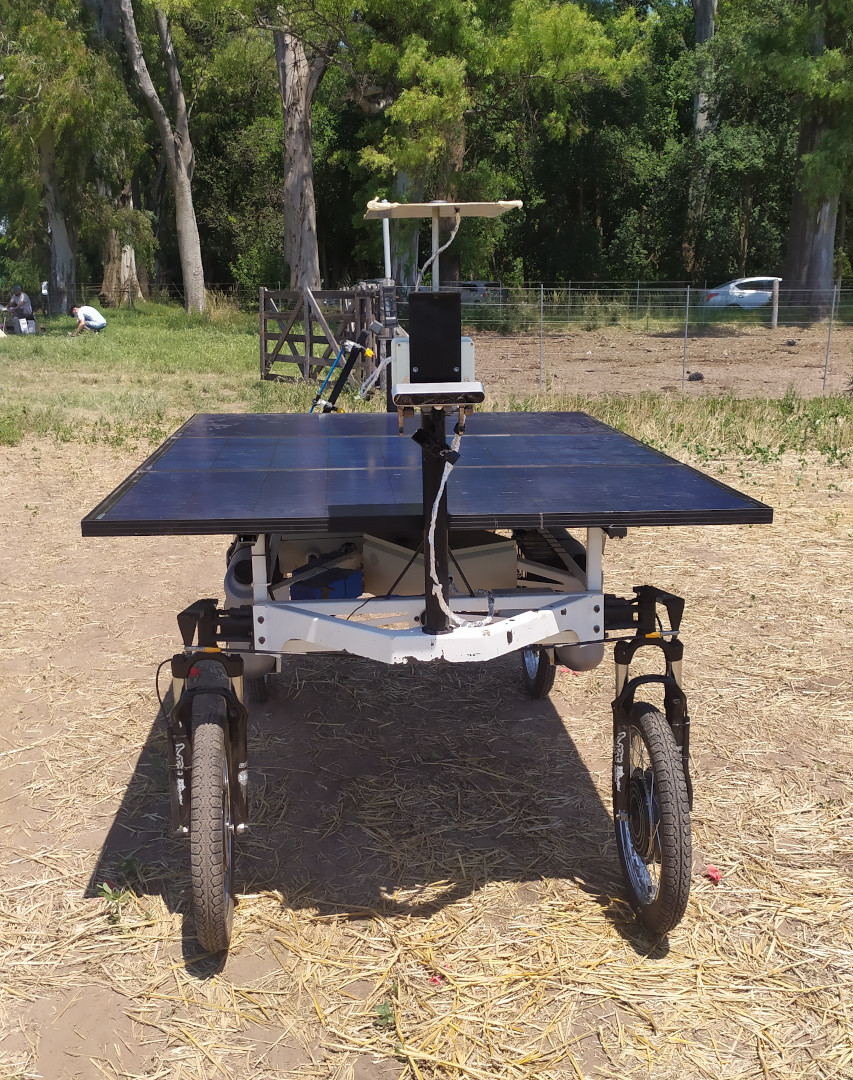
\includegraphics[width=0.4\columnwidth]{images/robot_front}}
    \hspace{0.1em}
    \subfloat[\label{subfig:robot_back}]{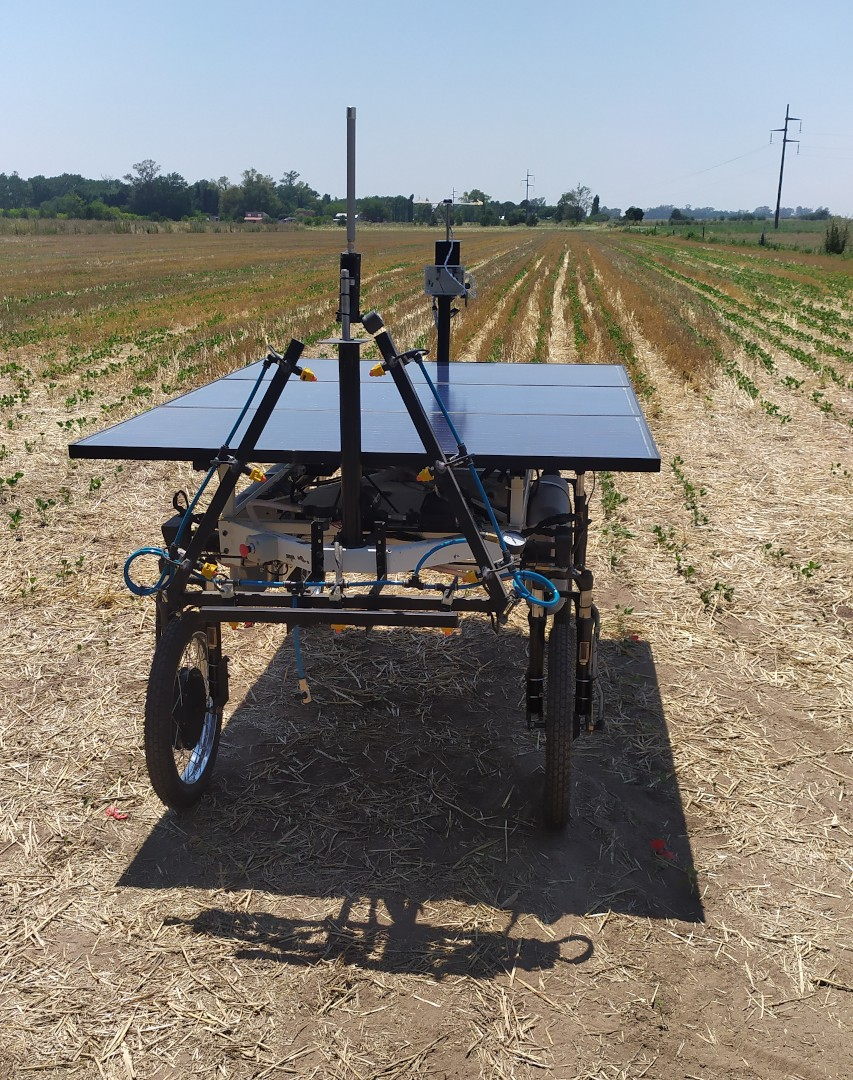
\includegraphics[width=0.4\columnwidth]{images/robot_back}}\\
    %\subfloat[]{\includegraphics[width=0.45\columnwidth]{example-image}}
    %\hspace{0.1em}
    \subfloat[\label{subfig:trajectory}]{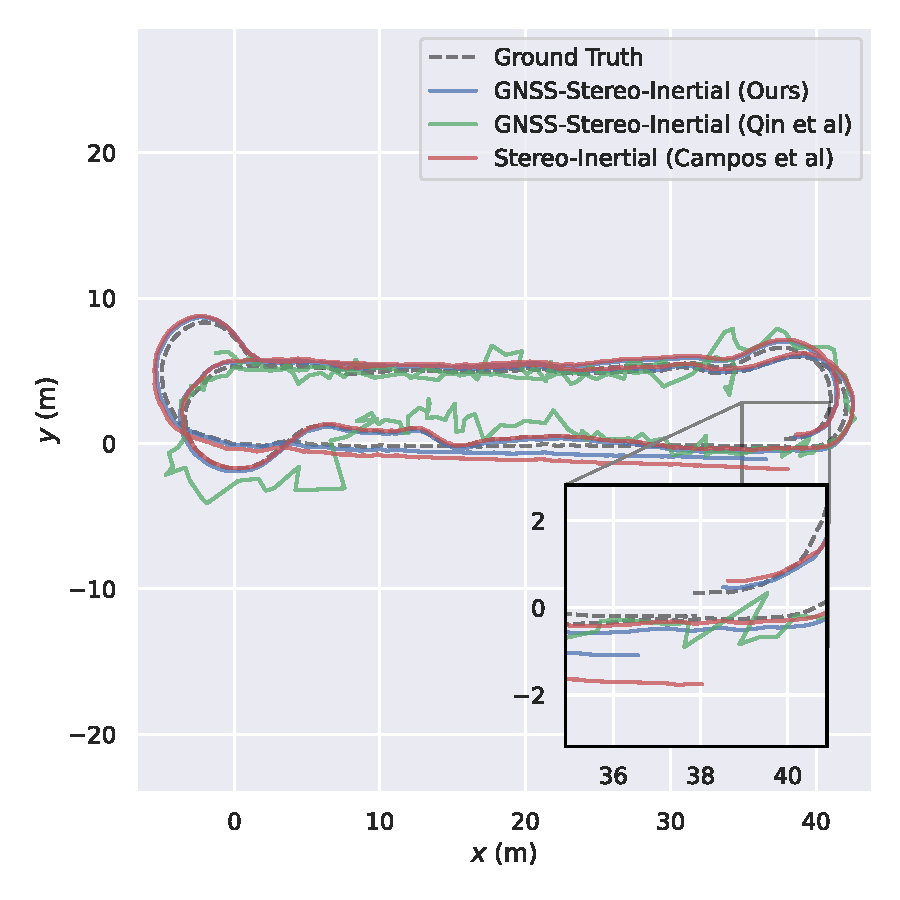
\includegraphics[width=.9\columnwidth]{images/zavalla_a.pdf}}
    \caption{\protect\subref{subfig:robot_front} and \protect\subref{subfig:robot_back}: Frontal and back views of our field robot and the arable field environment in which we navigate. \protect\subref{subfig:trajectory}: Trajectory estimated by our GNSS-stereo-inertial SLAM framework, along with GNSS-RTK ground truth,  visual-inertial ORB-SLAM3 \cite{campos2021orbslam3} and VINS-Fusion \cite{qin2019general}}
    \label{fig:teaser_image}
\end{figure}

Over the last decades, several agricultural tasks such as sowing, weed detection and removal or harvesting are being progressively automated targeting sustainable and environmentally friendly production. The use of autonomous robots in an agricultural environment has gained relevance, as it enables an efficient use of resources \cite{carelli2013agriculturalrobotics, wouter2014harvesting}. In general, in order to fully automate these and other agricultural tasks, the robot needs to know its pose relative to the environment in which it is navigating. 

A localization system must have a very high degrees of robustness and accuracy for a mobile robot to navigate safely without damaging the environment or itself. For most environments and tasks, a single sensor may not offer a sufficiently reliable robot pose estimate. As a few illustrative examples, GNSS sensors in outdoor environments do not accumulate error (drift) but they present considerable variance in their global position readings and may suffer frequent signal loss. State-of-the-art methods based on visual sensors perform badly if images have insufficient or repetitive textures, which is common in agricultural environments. Lighting can also be a problem if it is insufficient or excessive, and abrupt robot motion can cause image blur that degrades the estimation performance. Finally, interoceptive sensors that measure the internal state of the robot, such as the encoders in the wheel motors or inertial measurement units (IMU), are accurate for short-term motion estimation but drift after a few metres. Summing up, as all sensors have different and complementary advantages and disadvantages, it is essential for field robotics to properly fuse the measurements of multiple sensors to achieve robust and accurate pose estimates. This is particularly relevant to allow the robot to navigate over long periods of time (long-term navigation) and to keep the error bounded locally and globally.


SLAM, standing for Simultaneous Localization and Mapping, stands for the set of methods targeting global localization and mapping from a set of onboard sensors in a mobile agent \cite{cadena2016past}. A large number of visual-inertial SLAM pipelines have been proposed in the last decade \cite{mur2017visual,qin2018vins,campos2021orbslam3}. Many of them demonstrate high accuracy and robustness in indoor and urban environments. However, when it comes to the agricultural environment, they present problems in correctly estimating the pose of the robot. Among others, agricultural environments are challenging for visual navigation due to insufficient and/or repetitive texture and direct sunlight. Adding inertial measurements provides a slight improvement in the estimation. Nevertheless, as shown in \cite{cremona2022evaluation}, state-of-the-art visual-inertial systems accumulate significant errors after navigating a few minutes on arable lands. Robust SLAM systems such as ORB-SLAM3 \cite{campos2021orbslam3} can eliminate drift when revisiting already mapped places, but the so-called loop closing offers a poor performance on agricultural fields due to insufficiently discriminative visual appearances. A reasonable alternative, that we use in this work, is to employ measurements from global positioning sensors such as GNSS to allow the robot to navigate for long periods without accumulating drift.

This paper presents a GNSS-stereo-inertial SLAM implementation that fuses GNSS, visual and inertial measurements using a tightly-coupled approach. Specifically, we extend the state-of-the-art ORB-SLAM3 \cite{campos2021orbslam3} with GNSS factors. The global positioning measurements are incorporated into the mapping thread, so that it performs periodic corrections in the local map and hence also correct the current camera pose in the tracking thread. In this manner, we can achieve drift-less trajectories without depending on the ability of the system to close loops based on visual appearance. We evaluated our implementation on the agricultural dataset known as Rosario Dataset \cite{pire2019rosario} and an additional in-house dataset, which contains data from a wheeled robot in a soybean field (see Figure \ref{subfig:robot_front}-\ref{subfig:robot_back} for a picture of our robot). In both cases, we show how our implementations is able to effectively fuse GNSS readings outperforming the original stereo-inertial ORB-SLAM3. The contribution of the work can be summarized as follows:
\begin{itemize}
    \item Implementation of a GNSS-Stereo-Inertial framework.
    \item Evaluation of our GNSS-Stereo-Inertial framework tightly-coupled fusion in agricultural environments, incorporating real conventional GNSS measurements instead of simulated ones, which are rarely included in evaluations of state-of-the-art approaches.
    \item Public release of our implementation as open-source\footnote{\href{https://github.com/CIFASIS/gnss-stereo-inertial-fusion}{\nolinkurl{https://github.com/CIFASIS/gnss-stereo-inertial-fusion}}} , in order to facilitate its usage, extensions and comparisons and evaluations by the robotics community.
\end{itemize}

The article is organized as follows: Section~\ref{sec:related} discusses related work on multi-modal sensor fusion. In  Section~\ref{sec:method}, we describe the proposed GNSS-Stereo-Inertial framework. In Section~\ref{sec:experiments}, we present and discuss the experimental results of our GNSS-Stereo-Inertial implementation on real data in an agricultural field. Finally, we present our conclusions in Section~\ref{sec:conclusions}.


\section{Related Work}
\noindent\textbf{3D reconstruction from a single image.} 
Reconstructing various objects from a single image has been well studied~\cite{barron2014shape, wang2018pixel2mesh, wu2018learning}. They can produce high-quality 3D models of cars, planes, tables, and human body~\cite{saito2019pifu, saito2020pifuhd}. The main challenge is how to best recover objects' details, how to represent them with limited memory, and how to generalize to more diverse objects. However, all these methods rely on learning priors specific to a certain object class or instance, typically from 3D supervision, and can therefore not work for full scene reconstruction. Apart from these reconstructing objects works, several works focus on scene reconstruction~\cite{Xu_2023_ICCV} from a single image. Saxena~\etal~\cite{saxena2008make3d} construct the scene based on the assumption that the whole scene can be segmented into several small planes. With planes' orientation and location, the 3D structure can be represented. Recently, LeReS~\cite{leres} propose to use a strong monocular depth estimation model to do scene reconstruction. However, they can only recover the shape up to a scale. 
Zhang~\etal~\cite{Zhang_2023_ICCV} recently  propose a zero-shot geometry-preserving depth estimation model that is capable of making depth predictions up to an unknown scale, without requiring  scale-invariant depth annotations for training. 
In contrast to these works, our method can recover the metric 3D structure.



\noindent\textbf{Supervised monocular depth estimation.}
After several benchmarks~\cite{silberman2012indoor, Geiger2013IJRR} are established, neural network based
methods~\cite{yuan2022new, Yin2019enforcing, bhat2021adabins} have dominated since then. Several approaches regress the continuous depth from the aggregation of information in an image~\cite{eigen2014depth}. As depth distribution corresponding to different RGBs can vary to a large extent, some methods~\cite{Yin2019enforcing, 
bhat2021adabins}
discretize the depth and formulate this problem to a classification~\cite{yin2021virtual},  
which often achieves better performance. %
The generalization issue of deep models for 3D metric recovery   
is related to two problems. 
The first one is to generalize to diverse scenes, while 
the other 
one is how to predict accurate metric information under various camera settings. The first problem has been well addressed by recent methods. Some works~\cite{
xian2020structure, xian2018monocular, yin2021virtual} propose to construct a large-scale relative depth dataset, such as DIW~\cite{chen2016single} and OASIS~\cite{chen2020oasis}, and then they target learning the relative relations. However, the relative depth loses geometric structure information.
To improve the recovered geometry quality, 
learning affine-invariant depth methods, such as MiDaS~\cite{Ranftl2020}, LeReS~\cite{leres}, and HDN~\cite{ 
zhang2022hierarchical} are proposed. 
By mixing large-scale data, 
state-of-the-art performance and the generalization over scenes are improved continuously. 
Note that by design, these methods are unable to recover 
the metric information.
How to achieve both strong generalization and accurate metric information over diverse scenes is the key problem that
we attempt to tackle. 

\noindent\textbf{Large-scale data training.}
Recently, various natural language problems and computer vision problems~\cite{
yin2022devil, radford2021learning, lambert2020mseg} have achieved impressive progress with large-scale data training. CLIP~\cite{radford2021learning} is a promising classification model, which is trained on billions of paired image and language descriptions data. It achieved state-of-the-art performance over several classification benchmarks by zero-shot testing. 
For depth prediction, large-scale data training has been widely applied. Ranft~\etal~\cite{Ranftl2020} mixed over 2 million data in training, LeReS~\cite{yin2022towards} collected over $300$ thousands data, Eftekhar~\etal~\cite{eftekhar2021omnidata} also merged millions of data to build a strong depth prediction model. %







\section{Method}
This section presents the technical aspects of our implementation. Firstly, we introduce the notation and conventions adopted that are necessary to fully detail the model of our GNSS factor. Later, we briefly introduce ORB-SLAM3 \cite{campos2021orbslam3}, the state-of-the-art framework Visual-Inertial SLAM that we use in our method. We refer the reader to the original ORB-SLAM3 publication for the full details on such framework. Finally, we detail the formulation of our GNSS factor.

\subsection{Notation}
Figure~\ref{fig:frames} shows the coordinate frames used in this work. $\worldCoordSystem$ represents the world frame and $\bodyCoordSystem$ represents the body frame, that we place in the IMU sensor. $\vec{a}^{S}$ represents the coordinates of a geometry entity $\vec{a}$ with respect to the reference frame $S$. $\rotationCoord{\worldCoordSystem}{\bodyCoordSystem} \in SO(3)$ refers to the rotation of $\bodyCoordSystem$ with respect to $\worldCoordSystem$, and $\translationCoord{\worldCoordSystem}{\bodyCoordSystem} \in \mathbb{R}^3$ represents the translation of the reference frame $\bodyCoordSystem$ expressed in the frame $\worldCoordSystem$. The rigid transformation formed by the rotation $\rotationCoord{\worldCoordSystem}{\bodyCoordSystem}$ and the translation $\translationCoord{\worldCoordSystem}{\bodyCoordSystem}$ is denoted as $\rigidTransformCoord{\worldCoordSystem}{\bodyCoordSystem} \in SE(3)$, and transforms points in homogeneous coordinates from the reference frame ${\bodyCoordSystem}$ to the reference frame ${\worldCoordSystem}$. For global positioning measurements, $\translationCoord{\bodyCoordSystem}{\firstGPSCoordSystem} \in \mathbb{R}^3$ is the position of the GNSS antenna in the body frame, and is assumed to be known from a calibration stage. All GNSS measurements are transformed to the local Cartesian frame that we denote as ${\coordIndex{\firstGPSCoordSystem}{0}}$. We detail below how we choose such reference frame.

\begin{figure}[!t]
    \centering
    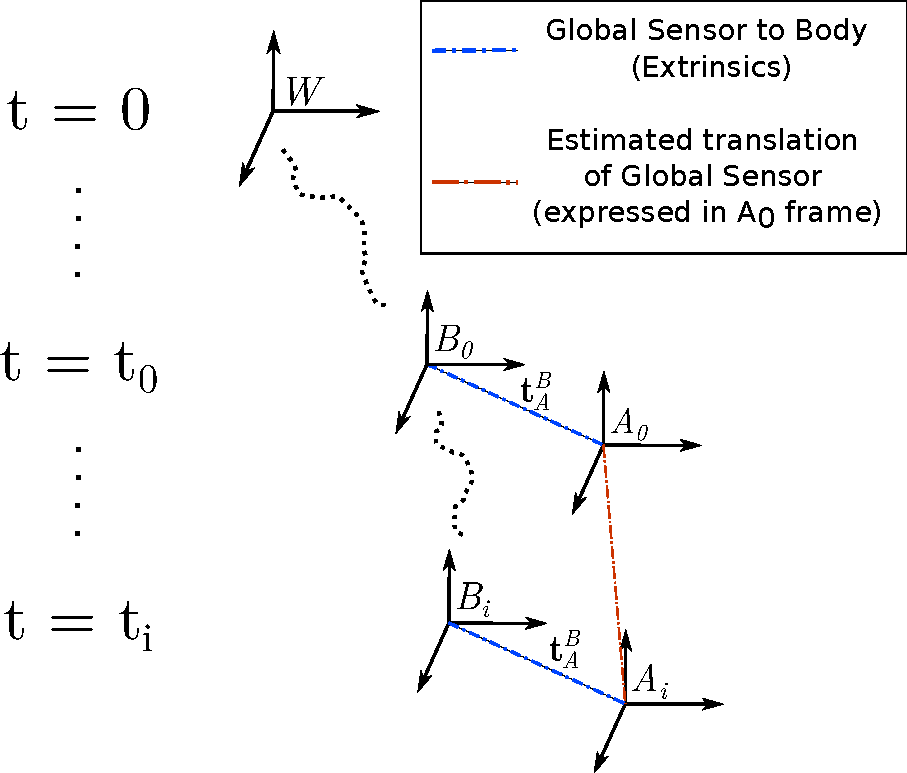
\includegraphics[width=\linewidth]{images/frames.pdf}
    \caption{Reference Frames used in this work. The position of the GNSS antenna in the body frame is represented with a translation and shown with a blue line, and can be obtained from the calibration of the system. The red line represents the estimated translation of the GNSS antenna from time $t_0$ to time $t_i$. This 3D vector is compared with the GNSS measurements in the GNSS error residual $\mathbf{r}_{\mathcal{G}_{i}}$. Both vectors are expressed in ${\coordIndex{\firstGPSCoordSystem}{0}}$ frame.}
    \label{fig:frames}
\end{figure}

\subsection{ORB-SLAM3}
ORB-SLAM3 is a state-of-the-art visual-inertial SLAM framework evolved from ORB-SLAM2 \cite{mur2017orb} and ORB-SLAM-VI \cite{mur2017visual}. With respect to ORB-SLAM-VI, ORB-SLAM3 proposes a substantially more robust inertial initialization based on maximum-a-posteriori estimates. As it is common in current SLAM systems, the processing is split into multiple threads to exploits multi-core architectures. Specifically, ORB-SLAM3 implements a tracking thread, a local mapping thread and a loop closure and map merging thread. The tracking thread estimates the pose of the current frame by minimizing the reprojection error and incorporating IMU constraints into the optimization by pre-integration \cite{forster2017onmanifold}. It also contains the heuristics for deciding whether a frame becomes a keyframe. The mapping thread main task is a visual-inertial bundle adjustment on a sliding window of keyframes, although it also performs auxiliary map management tasks such as point and keyframe culling. Finally, the loop closure and map merging thread ensures the global consistency of large maps by recognizing revisited places and correcting the drift, and joining separate maps if a common overlap is detected.

From the results in \cite{cremona2022evaluation}, ORB-SLAM3 presents an acceptable accuracy in arable lands for short camera trajectories, but long-term navigation is still challenging. The authors propose a novel loop closure algorithm to correct the drift. However, even with such improvement, loop closure keeps being challenging due to the similarity in appearance of the local visual features. As a result, visual SLAM systems may accumulate drift when loop closures are not detected or the estimation may be corrupted by false loop detections.

\subsection{GNSS-Stereo-Inertial Fusion}
In this work, we formulate a tightly-coupled approach for fusing visual, inertial and GNSS data. Firstly, GNSS measurements are associated to the timestamp of a keyframe according to their temporal proximity. If there is a keyframe with a temporal difference under a specific threshold, the GNSS constraint is set to this keyframe. GNSS readings that are not close in time to any keyframe are discarded (see an illustration of this approach in Figure~\ref{fig:association}). While this is an approximation, we found that, given the high variance of conventional GNSS, a sufficiently small threshold and appropriate keyframe management policy makes its effect negligible. 

The first GNSS reading that is associated with a keyframe determines the position of $\coordIndex{\firstGPSCoordSystem}{0}$, the Cartesian frame for our global position measurements (see Figure~\ref{fig:frames}). We choose $\coordIndex{\firstGPSCoordSystem}{0}$ as a East-North-Up (ENU) local Cartesian frame. The subsequent GNSS measurements are transformed to be expressed in $\coordIndex{\firstGPSCoordSystem}{0}$, and we refer to them as $\noisyMeasurement_{i}$, where $t_i$ is the timestamp of the corresponding keyframe. This is done once the IMU is initialized. If the map is reset, the process of selecting $\coordIndex{\firstGPSCoordSystem}{0}$ is repeated. 

\begin{figure}[!t]
    \centering
    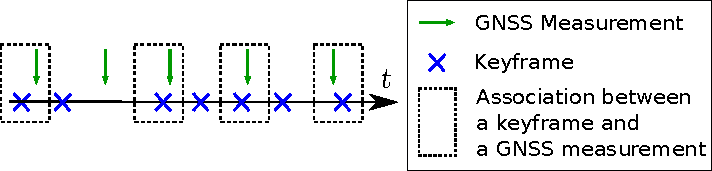
\includegraphics[width=\linewidth]{images/association.pdf}
    \caption{Temporal association between keyframes and GNSS measurements. %Keyframes are depicted with blue crosses on the temporal line and GNSS measurements are depicted with green arrows. 
    GNSS measurements are discarded if they are further than specific temporal threshold from any keyframe.}
    \label{fig:association}
\end{figure}

Our GNSS-Stereo-Inertial fusion is done in the local bundle adjustment of a sliding window of keyframes and 3D points observed from them. Figure~\ref{fig:graph} shows the factor graph corresponding to such optimization. The state variables to optimize are $\mathcal{X} = \{\mathcal{X}_{B}, \mathcal{L}\}$, where $\mathcal{X}_{B} = [\systemState_{1},\dots,\systemState_{i},\dots,\systemState_{N}]$ is the set of sensor states for a window covering the last $N$ keyframes and $\mathcal{L}= [\mathbf{y}_{1},\dots,\mathbf{y}_{j},\dots,\mathbf{y}_{M}]$ is the set of landmarks states that were measured during those last $N$ keyframes. The sensor state $\systemState_{i}$ at the time instant $i$ is
%
\begin{equation}
    \systemState_{i} = [\rigidTransformCoord{\worldCoordSystem}{\coordIndex{\bodyCoordSystem}{i}}, \coordIndex{\linearVelocity}{i}^\top, \bias_{a_i}^\top, \bias_{g_i}^\top],
\end{equation}
%
which contains the sensor rigid transformation with respect to the world frame $\rigidTransformCoord{\worldCoordSystem}{\coordIndex{\bodyCoordSystem}{i}} \in SO(3)$, its local velocity $\coordIndex{\linearVelocity}{i} \in \mathbb{R}^3$ and the accelerometer and gyroscope bias $\bias_{a_i} \in \mathbb{R}^3$ and $\bias_{g_i} \in \mathbb{R}^3$. Landmarks are represented by their Euclidean coordinates in the world frame, i.e., $\mathbf{y}_{j} = [X^W, Y^W, Z^W]^\top \in \mathbb{R}^3$

In comparison to ORB-SLAM3, a GNSS error term is added to the cost function. Note that, as shown in Figure~\ref{fig:association}, some keyframes may not have an associated GNSS measurement. %Then the cost function to be minimized results in:
Then, our GNSS-Stereo-Inertial mapping optimization can be stated as follows
%
\begin{equation}
\begin{split}
    \hat{\mathcal{X}} = \argmin_{\mathcal{X}} \left( \sum_{i=1}^N \lVert \mathbf{r}_{\mathcal{I}_{i-1,i}}  \rVert^2_{\Sigma_{\mathcal{I}_{i-1,i}}^{-1}} +\right. \\ 
    \left. + \sum_{j=1}^M \sum_{i \in \mathcal{K}_j} \rho \left( \lVert \mathbf{r}_{\mathcal{V}_{ij}} \rVert_{\Sigma_{{V}_{ij}}^{-1}} +\right) \right. \\
    \left. + \sum_{i \in \mathcal{N}^*} \rho \left( \lVert \mathbf{r}_{\mathcal{G}_{i}} \rVert_{\Sigma_{\mathcal{G}_{i}}^{-1}} +\right) \right),
\end{split}
\end{equation}
%
where $\mathcal{N}^*$ is the set of keyframes that have an associated GNSS measurement. The three addends correspond, respectively, to the inertial, visual and GNSS constraints. For completitude we will detail the three of them, although the first two are used exactly as proposed in ORB-SLAM3 and the third one is our novel contribution.

The inertial residual is defined as follows
%
\begin{equation}
\mathbf{r}_{\mathcal{I}_{i-1,i}} = [\mathbf{r}_{\Delta \mathbf{R}_{i-1,i}}^\top, \mathbf{r}_{\Delta \mathbf{v}_{i-1,i}}^\top, \mathbf{r}_{\Delta \mathbf{p}_{i-1,i}}^\top]^{\top},
\end{equation}
%
where $\mathbf{r}_{\Delta \mathbf{R}_{i-1,i}}$, $\mathbf{r}_{\Delta \mathbf{v}_{i-1,i}}$ and $\mathbf{r}_{\Delta \mathbf{p}_{i-1,i}}$ correspond to orientation, velocity and position residuals that have the following form
%
\begin{equation}
\footnotesize
\begin{aligned}
\mathbf{r}_{\Delta \mathbf{R}_{i-1,i}} &= \log \left( \Delta \mathbf{R}_{i-1,i}^\top \mathbf{R}_{i-1}^\top \mathbf{R}_{i} \right) \\
\mathbf{r}_{\Delta \mathbf{v}_{i-1,i}} &= \mathbf{R}_{i}^\top \left( \mathbf{v}_{i} - \mathbf{v}_{i-1} - \mathbf{g}\Delta t_{i-1,i} \right) - \Delta \mathbf{v}_{i-1,i} \\
\mathbf{r}_{\Delta \mathbf{p}_{i-1,i}} &= \mathbf{R}_{i}^\top \left( \mathbf{p}_{i} - \mathbf{p}_{i-1} - \mathbf{v}_{i} \Delta t_{i-1,i} - \frac{1}{2}\mathbf{g}\Delta t_{i-1,i}^2 \right) - \\ & \ \ \ - \Delta \mathbf{p}_{i-1,i}.
\end{aligned}
\end{equation}
%
The terms denoted as $\Delta \mathbf{R}_{i-1,i}$, $\Delta \mathbf{v}_{i-1,i}$ and $\Delta \mathbf{p}_{i-1,i} $ come from the preintegration of the IMU readings between the time instants $i-1$ and $i$, and are computed together with their on-manifold covariance $\Sigma_{\mathcal{I}_{i-1,i}}$ according to \cite{forster2017onmanifold}. $\mathbf{g}$ stands for the gravity direction, which is set at the system bootstrapping.

The visual residual $\mathbf{r}_{\Delta \mathbf{v}_{i-1,i}}$ is
%
\begin{equation}
    \mathbf{r}_{\mathcal{V}_{ij}} = \mathbf{u}_{ij} - \pi\left( \rigidTransformCoord{C}{\bodyCoordSystem} \rigidTransformCoord{\worldCoordSystem-1}{\bodyCoordSystem} \tilde{\mathbf{y}}_{j} \right),
\end{equation}
%
where $ \tilde{\mathbf{y}}_{j}$ stands for the homogeneous representation of the $j^{th}$ landmark, $\pi(\cdot)$ for the pinhole projection model of a 3D point in homogeneous coordinates in a stereo image, and $\mathbf{u}_{ij}$ the measured image coordinates of the $j^{th}$ landmark in the $i^{th}$ stereo keyframe. The visual covariance of image landmarks $\Sigma_{\mathcal{V}_{ij}}$ is set to the standard 1-pixel standard deviation isotropic Gaussian.

Finally, the GNSS error residual is
%
\begin{equation}
\footnotesize
\mathbf{r}_{\mathcal{G}_{i}} = \noisyMeasurement_{i} -  \rotationCoord{\coordIndex{\firstGPSCoordSystem}{0}}{\worldCoordSystem}\left(\rotationCoord{\worldCoordSystem}{\coordIndex{\bodyCoordSystem}{i}}\translationCoord{\bodyCoordSystem}{\firstGPSCoordSystem} + \translationCoord{\worldCoordSystem}{\coordIndex{\bodyCoordSystem}{i}} - \left(\rotationCoord{\worldCoordSystem}{\coordIndex{\bodyCoordSystem}{0}}\translationCoord{\bodyCoordSystem}{\firstGPSCoordSystem} + \translationCoord{\worldCoordSystem}{\coordIndex{\bodyCoordSystem}{0}} \right)\right).
\end{equation}
%
The second term represents the translation vector of the global sensor (in this case, the GNSS antenna) at time instant $i$ in the reference frame $\coordIndex{\firstGPSCoordSystem}{0}$, as can be seen in Figure~\ref{fig:frames}. $\rotationCoord{\worldCoordSystem}{\coordIndex{\bodyCoordSystem}{0}}$ and $\translationCoord{\worldCoordSystem}{\coordIndex{\bodyCoordSystem}{0}}$, which are the relative rotation and translation between the body and the world frame at time $t_0$, are kept constant during the optimization. $\rotationCoord{\coordIndex{\firstGPSCoordSystem}{0}}{\worldCoordSystem}$ is computed by aligning  the first 20 GNSS measurements  with the poses estimated by ORB-SLAM3 in the same time period using Umeyama's method \cite{umeyama1991least}. After estimating this rotation, it is kept fixed during the whole optimization process. The covariance matrix $\Sigma_{\mathcal{G}_{i}}$ is set from the specifications sheet of our GNSS device in each Cartesian axis
%
\begin{equation}
\Sigma_{\mathcal{G}_{i}} = \begin{bmatrix}
\sigma_x^{2} & 0 & 0\\
0 & \sigma_y^{2} & 0 \\
0 & 0 & \sigma_z^{2}
\end{bmatrix}.
\end{equation}
%
This covariance matrix is defined relative to a tangential plane through the GNSS reported position. The values are expressed in ENU frame. Finally, the Jacobian with respect to the pose error state is defined as
%
\begin{equation}
\frac{\partial \mathbf{r}_{\mathcal{G}_{i}}}{\partial \delta \rigidTransformCoord{\worldCoordSystem}{\coordIndex{\bodyCoordSystem}{i}}} = \left[ \rotationCoord{\coordIndex{\firstGPSCoordSystem}{0}}{\worldCoordSystem}  \rotationCoord{\worldCoordSystem}{\coordIndex{\bodyCoordSystem}{i}} \left[ \translationCoord{\bodyCoordSystem}{\firstGPSCoordSystem}\right]^{\times} \quad -\rotationCoord{\coordIndex{\firstGPSCoordSystem}{0}}{\worldCoordSystem}  \right],
\end{equation}

where $\delta$ indicates that the derivative is computed with respect to a right perturbation in the pose.

%
\begin{figure}[!tb]
    \centering
    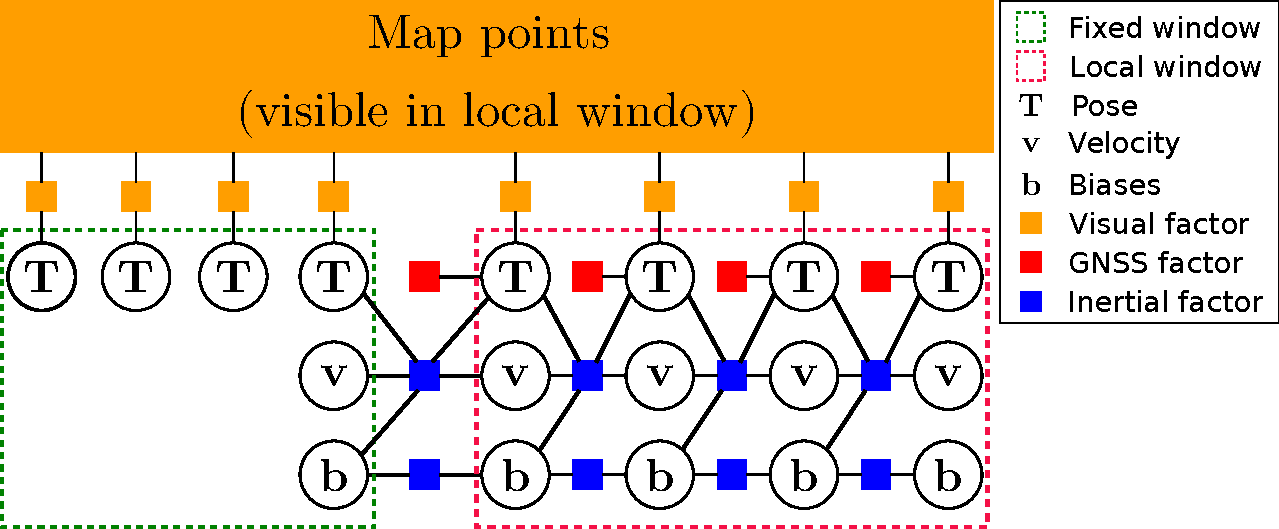
\includegraphics[width=\columnwidth]{images/graph.pdf}
    \caption{Factor Graph corresponding to the Local Bundle Adjustment of our GNSS-Stereo-Inertial SLAM. In comparison to ORB-SLAM3, a GNSS factor (in red) is added to the cost function. The Local Window is composed by the $N$ last keyframes.}
    \label{fig:graph}
\end{figure}


\section{Experiments}

\noindent\textbf{Dataset details.}
\label{sec:data}
We collect $11$ public RGB-D datasets, and over $8$ million data for training. It spreads over diverse indoor and outdoor scenes. Note that all datasets have provided %
camera intrinsic parameters. Apart from the test split of training datasets, we collect $7$ unseen datasets for robustness and generalization evaluation. Details of employed data are reported in the supplementary materials.  



\noindent\textbf{Implementation details.}
We employ an UNet architecture with the ConvNext-large~\cite{liu2022convnet} backbone. ImageNet-22K pre-trained weights are used for initialization. We use AdamW with a batch size of $192$, an initial learning rate $0.0001$ for all layers, and the polynomial decaying method with the power of $0.9$. We train our final model on $48$ A100 GPUs for $500$K iterations. Following the DiverseDepth~\cite{yin2021virtual}, we balance all datasets in a mini-batch to ensure each dataset accounts for an almost equal ratio. During training, images are processed by the canonical camera transformation module, flipped horizontally with a $50\%$ chance, and then randomly cropped into 
$512 \times 960$ pixels. For the ablation experiments, training settings are different as we sample $5000$ images from each dataset for training. We trained on $8$ GPUs for $150$K iterations.










\noindent\textbf{Evaluation details.}
a) To show the robustness of our metric depth estimation 
method, we test on 8 zero-shot benchmarks, including NYUv2~\cite{silberman2012indoor}, KITTI~\cite{Geiger2013IJRR}, NuScenes~\cite{caesar2020nuscenes}, 7-scenes~\cite{shotton2013scene}, iBIMS-1~\cite{koch2018evaluation}, DIODE~\cite{vasiljevic2019diode}, ETH3D~\cite{schops2017multi}. Following previous works~\cite{yuan2022new}, absolute relative error (AbsRel),  the accuracy under threshold ($\delta_{i} < 1.25^{i}, i=1, 2, 3$), root mean squared error (RMS), root mean squared error in log space (RMS\_{log}), and log10 error (log10) metrics are employed. 
b) Furthermore, %
we also follow current affine-invariant depth benchmarks~\cite{leres, zhang2022hierarchical} (Tab. \ref{Table: generalization evaluation.}) to evaluate the generalization ability on $5$ zero-shot datasets, \textit{i.e.},  NYUv2, DIODE, ETH3D, ScanNet~\cite{dai2017scannet}, and KITTI. We mainly compare with large-scale data trained models. Note that in this benchmark we follow existing methods to apply the scale shift alignment before evaluation. 
c) To evaluate our metric 3D reconstruction quality, we randomly sample 9 unseen scenes from NYUv2 and use colmap~\cite{schoenberger2016mvs} to obtain the camera poses for multi-frame reconstruction. Chamfer $l_1$ distance and the F-score~\cite{knapitsch2017tanks} are used to evaluate the reconstruction accuracy. 
d) In dense-SLAM experiments, following Li~\etal~\cite{li2021generalizing}, we test on the KITTI odometry benchmark~\cite{Geiger2013IJRR} and evaluate the average translational RMS drift ($\%, t_{rel}$) and rotational RMS drift ($\degree/100m, r_{rel}$) errors~\cite{Geiger2013IJRR}.
Note that all these depth and reconstruction evaluations use the same trained model. 

\subsection{Zero-shot Generalization %
Test
}

\begin{table}[!t]
\caption{Quantitative comparison on NYUv2 and KITTI benchmarks. Both datasets are unseen to our model, but we can achieve comparable performance with state-of-the-art methods.}
\vspace{-1 em}
\scalebox{0.67}{
\begin{tabular}{r |cccccc}
\toprule[1pt]
\multicolumn{7}{c}{\textbf{NYUv2 Benchmark}} \\ \hline
\multirow{1}{*}{Method} & $\boldsymbol{\delta_{1}}$$\uparrow$ & $\boldsymbol{\delta_{2}}$$\uparrow$ & $\boldsymbol{\delta_{3}}$$\uparrow$ & \textbf{AbsRel}$\downarrow$ & \textbf{log10}$\downarrow$ & \textbf{RMS}$\downarrow$  \\ \hline
Li \etal.~\cite{li2017two}               & $0.788$    & $0.958$    & $0.991$  & $0.143$   & $0.063$    & $0.635$     \\
Laina \etal.~\cite{laina2016deeper}      & $0.811$    & $0.953$    & $0.988$  & $0.127$   & $0.055$    & $0.573$       \\
VNL ~\cite{Yin2019enforcing}            & $0.875$   & $0.976$    & $0.994$  & $0.108$   & $0.048$    & $0.416$    \\ 
TrDepth~\cite{yang2021transformers}     & $0.900$   & $0.983$    & $0.996$  & $0.106$  & $0.045$     & $0.365$   \\
Adabins~\cite{bhat2021adabins}         & $0.903$    & ${0.984}$  & $\underline{0.997}$  & $0.103$  & $0.044$     & $0.364$    \\
NeWCRFs~\cite{yuan2022new}              
& ${0.922}$  & $\boldsymbol{0.992}$  & $\boldsymbol{0.998}$ 
& $0.095$  & $0.041$     & $\underline{0.334}$   \\ \hline
Ours CSTM\_image    
& $\boldsymbol{0.925}$  & $0.983$  & $0.994$ 
& $\underline{0.092}$   & $\underline{0.040}$   & ${0.341}$  \\
Ours CSTM\_label    
& $\underline{0.944}$  & $\underline{0.986}$  & $0.995$ 
& $\boldsymbol{0.083}$   & $\boldsymbol{0.035}$   & $\boldsymbol{0.310}$  \\\hline
\hline
\multicolumn{7}{c}{\textbf{KITTI Benchmark}} \\ \hline \hline
\multirow{1}{*}{Method} & $\boldsymbol{\delta_{1}}$$\uparrow$ & $\boldsymbol{\delta_{2}}$$\uparrow$ & $\boldsymbol{\delta_{3}}$$\uparrow$ & \textbf{AbsRel} $\downarrow$ & \textbf{RMS} $\downarrow$ & \textbf{RMS\_log} $\downarrow$ \\ \hline
Guo \etal \cite{guo2018learning}  & $0.902$  & $0.969$  & $0.986$ & $0.090$ & $3.258$ & $0.168$    \\
VNL~\cite{Yin2019enforcing} & ${0.938}$   & ${0.990}$   & ${0.998}$  & ${0.072}$  & $3.258$      & ${0.117}$    \\ 
TrDepth~\cite{yang2021transformers}   & $0.956$  & $0.994$  & $0.999$   & $0.064$  & $2.755$  & $0.098$  \\
Adabins~\cite{bhat2021adabins} & $0.964$  & $0.995$  & $0.999$   & $\underline{0.058}$  & $2.360$  & $0.088$  \\
NeWCRFs~\cite{yuan2022new} 
& $\boldsymbol{0.974}$  & $\boldsymbol{0.997}$  & $\underline{0.999}$   & $\boldsymbol{0.052}$  & $\boldsymbol{2.129}$  & $\boldsymbol{0.079}$  \\ \hline
Ours CSTM\_image & 
$\underline{0.967}$   & $\underline{0.995}$   & $\boldsymbol{0.999}$  
& $0.060$  & ${2.843}$     & $\underline{0.087}$    \\ 
Ours CSTM\_label 
& ${0.964}$   & ${0.993}$   & ${0.998}$  
& $0.058$  & ${2.770}$     & ${0.092}$    \\ \hline
\toprule[1pt]
\end{tabular}\newline}
\label{table:errors cmp on NYUD-V2}
\vspace{-2 em}
\end{table}






\begin{table*}[]
\renewcommand\arraystretch{1.1}
\caption{Quantitative comparison of 3D scene reconstruction with LeReS~\cite{leres}, DPT~\cite{ranftl2021vision}, %
RCVD~\cite{kopf2021rcvd}, 
SC-DepthV2~\cite{bian2021tpami}, and a learning-based MVS method (DPSNet~\cite{im2019dpsnet}) on 9 unseen NYUv2 scenes. Apart from DPSNet and ours, other methods have to align the scale with ground truth depth for each frame. As a result, our reconstructed 3D scenes achieve the best performance.}
\vspace{-1 em}
\centering
\resizebox{.98\linewidth}{!}{%
  \centering
  \small 
  \setlength{\tabcolsep}{0.5mm}{\begin{tabular}{@{} r |rc|rc|rc|rc|rc|rc|rc|rc|rc@{}}
    \toprule
    \multirow{2}{*}{Method} & \multicolumn{2}{c|}{Basement\_0001a} & \multicolumn{2}{c|}{Bedroom\_0015} & \multicolumn{2}{c|}{Dining\_room\_0004} & \multicolumn{2}{c|}{Kitchen\_0008} & \multicolumn{2}{c|}{Classroom\_0004} & \multicolumn{2}{c|}{Playroom\_0002}  & \multicolumn{2}{c|}{Office\_0024} & \multicolumn{2}{c|}{Office\_0004} & \multicolumn{2}{c}{Dining\_room\_0033}\\
      & C-$l_1$$\downarrow$ & F-score $\uparrow$ & C-$l_1$$\downarrow$ & F-score $\uparrow$ & C-$l_1$$\downarrow$ & F-score $\uparrow$ & C-$l_1$$\downarrow$ & F-score $\uparrow$ & C-$l_1$$\downarrow$ & F-score $\uparrow$ & C-$l_1$$\downarrow$ & F-score $\uparrow$ &
      C-$l_1$$\downarrow$ & F-score $\uparrow$ & C-$l_1$$\downarrow$ & F-score $\uparrow$ & C-$l_1$$\downarrow$ & F-score $\uparrow$\\ \hline
    RCVD~\cite{kopf2021rcvd} & 0.364 & 0.276 
            & 0.074 & 0.582 &
             0.462 & 0.251 &
             0.053 & 0.620 &
              0.187 & 0.327 &
             0.791 & 0.187 &
             0.324 & 0.241  &
             0.646 & 0.217 &
             0.445 & 0.253 \\

    SC-DepthV2~\cite{bian2021tpami}  & 0.254 & 0.275 &
             0.064 & 0.547 &
             0.749 & 0.229 &
             0.049 & 0.624 &
              0.167 & 0.267 &
             0.426 & 0.263 &
             0.482 & 0.138  &
             0.516 & 0.244 &
             0.356 &0.247 \\

    DPSNet~\cite{im2019dpsnet} & 0.243 & 0.299 &
             0.195 & 0.276 &
             0.995 & 0.186 &
             0.269 & 0.203 &
             0.296 & 0.195 &
             0.141 & 0.485 &
             0.199 & 0.362  &
             0.210 & 0.462 &
             0.222 & 0.493 \\
              
    DPT~\cite{leres} & 0.698 & 0.251 &
             0.289 & 0.226 &
             0.396 & 0.364 &
             0.126 & 0.388 &
             0.780 & 0.193 & 
             0.605 & 0.269 &
             0.454 & 0.245  &
             0.364 & 0.279 &
             0.751 & 0.185 \\  
    LeReS~\cite{leres} & 0.081 & 0.555 &
             0.064 & 0.616 &
             0.278 & 0.427 &
             0.147 & 0.289 &
             \textbf{0.143} & \textbf{0.480} &
             0.145 & 0.503 &
             0.408 & 0.176  &
             0.096 & 0.497 &
             0.241 & 0.325 \\  \hline
    Ours & \textbf{0.042} & \textbf{0.736} &
             \textbf{0.059} & \textbf{0.610} &
             \textbf{0.159} & \textbf{0.485} &
             \textbf{0.050} & \textbf{0.645} &
             0.145 & 0.445 &
             \textbf{0.036} & \textbf{0.814} &
             \textbf{0.069} & \textbf{0.638}  &
             \textbf{0.045} & \textbf{0.700} &
             \textbf{0.060} & \textbf{0.663} \\

    \bottomrule
  \end{tabular}}}
  \label{tab: NYUD reconstruction cmp.}
\end{table*}

\begin{figure*}[]
\centering
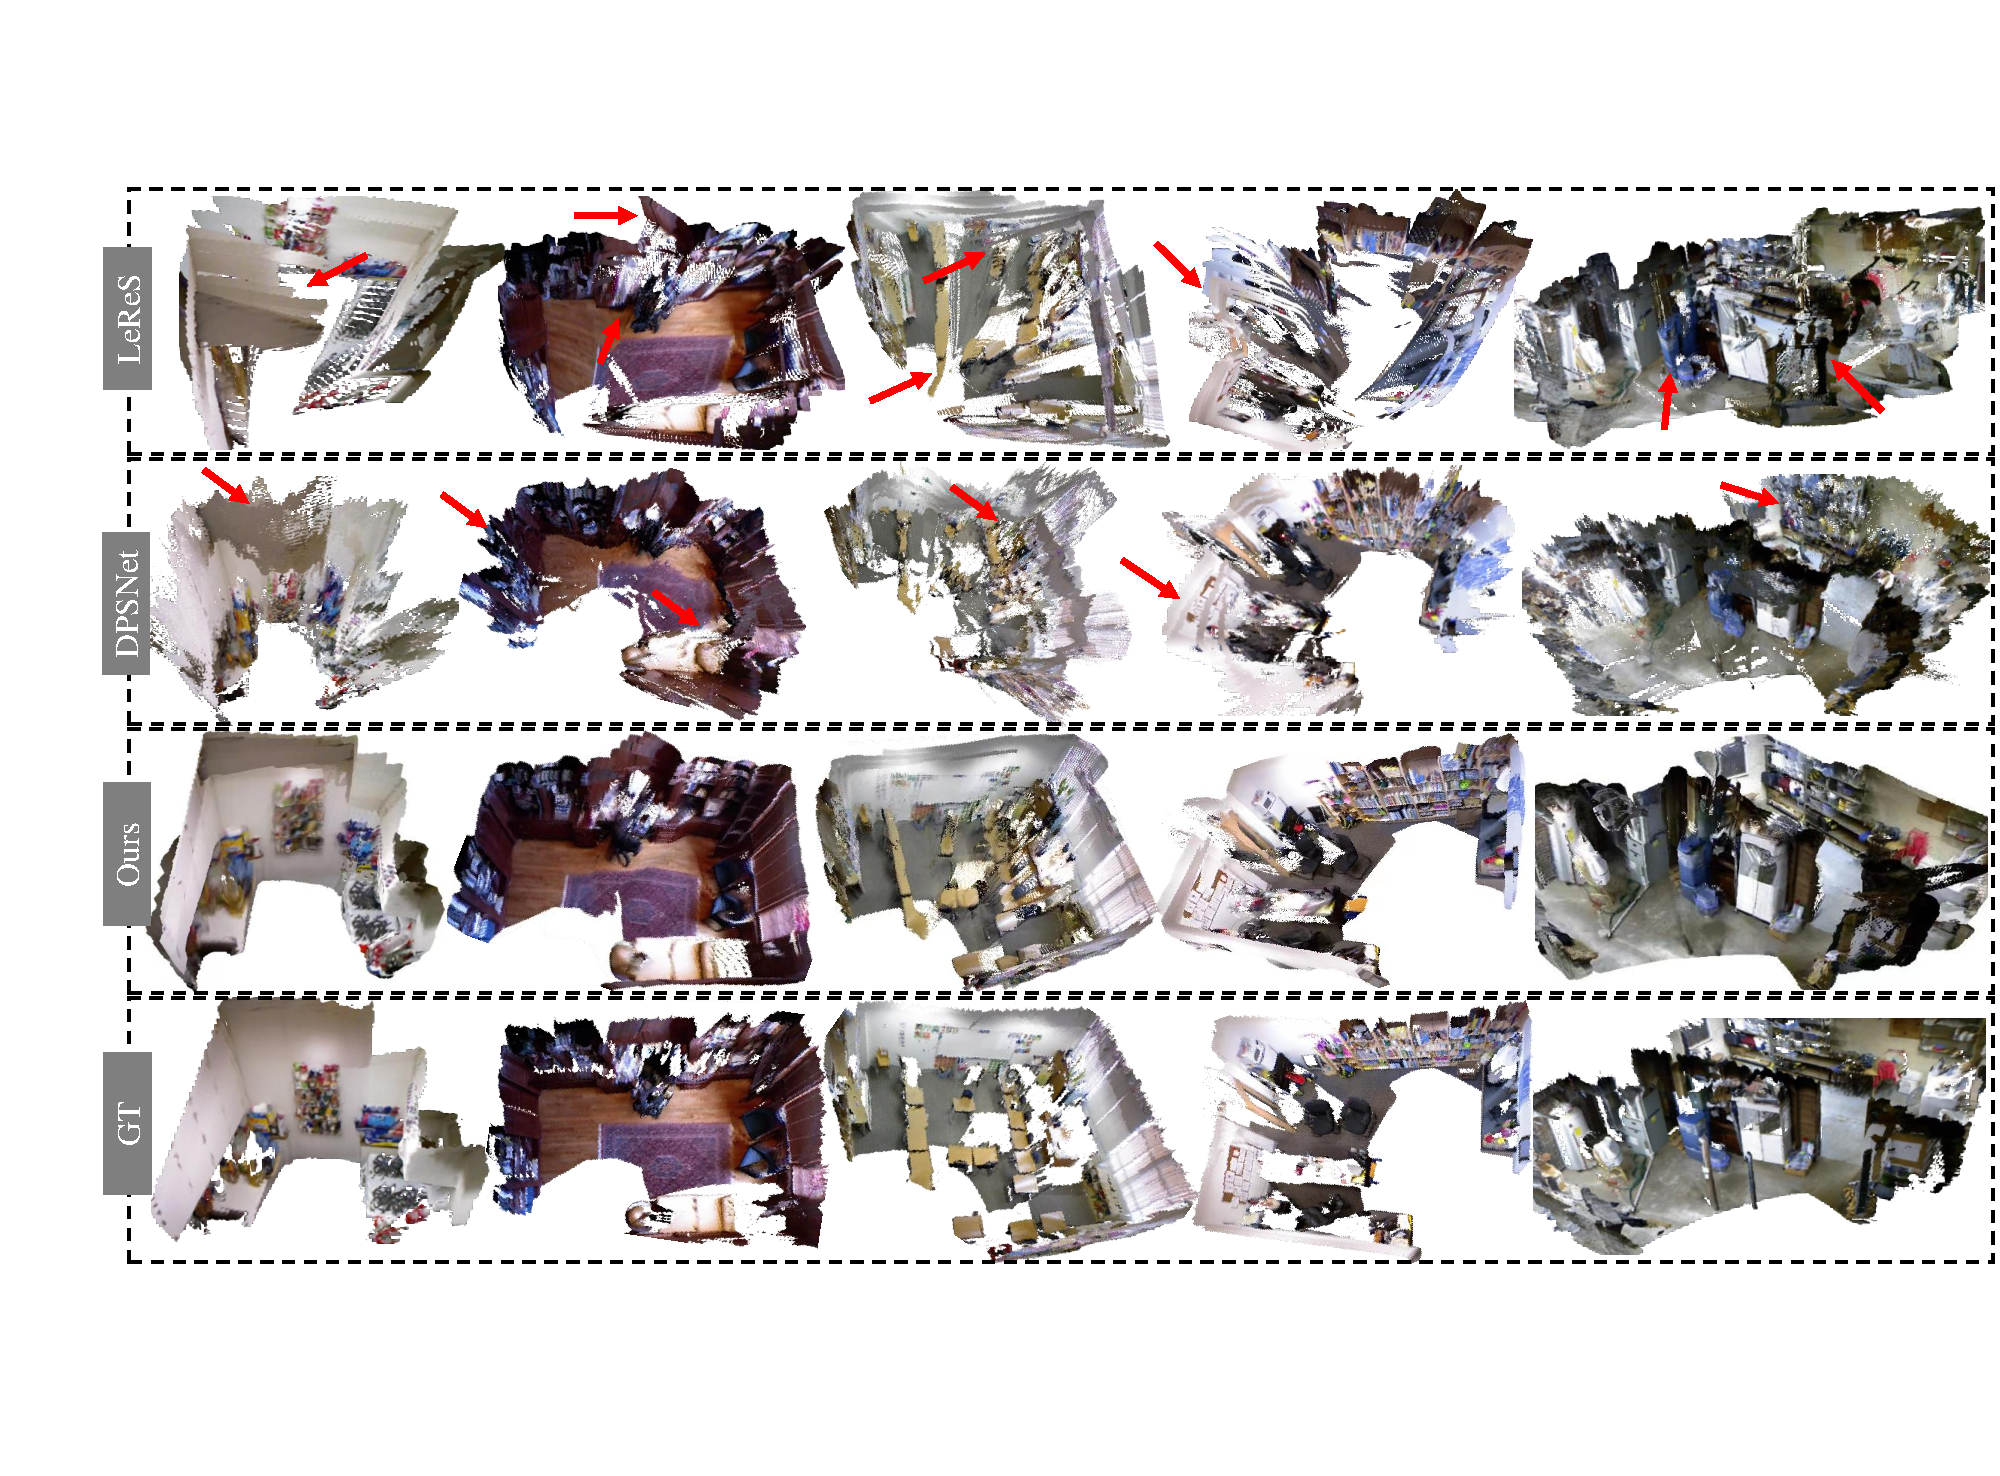
\includegraphics[width=0.95\textwidth]{./files/3dreconstruction.pdf}
\vspace{-1 em}
\caption{\textbf{Reconstruction of zero-shot scenes with multiple views.} We sample several NYUv2 scenes for 3D reconstruction comparison. As our method can predict accurate metric depth, thus all frame's predictions are  fused together for scene reconstruction. By contrast, LeReS~\cite{leres}'s depth is up to an unknown scale and shift, which causes noticeable distortions. DPSNet~\cite{im2019dpsnet} is a multi-view stereo method, which cannot work well on low-texture regions. }
\label{fig: visual nyud reconstruction cmp.}
\vspace{-1em}
\end{figure*}




\noindent\textbf{Evaluation on metric depth benchmarks.} To evaluate the accuracy of predicted metric depth, firstly,  we compare with state-of-the-art (SOTA) metric depth prediction methods on NYUv2~\cite{silberman2012indoor}, KITTI~\cite{geiger2012we}.
We use the same model to do %
all evaluations. %
Results are reported in Tab.~\ref{table:errors cmp on NYUD-V2}. Without any fine-tuning or metric adjustment,  we can achieve comparable performance with SOTA methods, which are trained on benchmarks for hundreds of epochs. %







Furthermore, We collect $6$ unseen datasets to do more metric accuracy evaluation. These datasets contain a wide range of indoor and outdoor scenes, including rooms, buildings, and driving scenes. The camera models are also various, e.g. 7scenes has a short focal length (around 500), while ETH3D is 2000. We mainly compare with the SOTA metric depth estimation methods and take their NYUv2 and KITTI models for indoor and outdoor scenes evaluation respectively. From Tab. \ref{table: metric eval on more datasets.}, we observe that although 7Scenes is similar to NYUv2 and NuScenes is similar to KITTI, existing methods face a noticeable performance decrease. In contrast, our model is more robust. %

\begin{table*}[]
\centering
 \caption{Quantitative comparison with SOTA metric depth methods on $6$ unseen benchmarks. For SOTA methods, we use their NYUv2 and KITTI models for indoor and outdoor scenes evaluation respectively, while we use the same model for all zero-shot testing. }
 \vspace{-1 em}
 \resizebox{0.9\linewidth}{!}{%
\begin{tabular}{l|lll|lll}
\toprule[1pt]
\multirow{2}{*}{Method}        & DIODE(Indoor) & iBIMS-1 & 7Scenes      & DIODE(Outdoor)      & ETH3D      & NuScenes     \\
        & \multicolumn{3}{c|}{Indoor scenes (AbsRel$\downarrow$/RMS$\downarrow$)}  & \multicolumn{3}{c}{Outdoor scenes (AbsRel$\downarrow$/RMS$\downarrow$)} \\ \hline
Adabins~\cite{bhat2021adabins}  
         &  0.443 / 1.963       
         &0.212 / 0.901         
         & 0.218 / 0.428 
         &0.865 / 10.35                     
         &1.271 / 6.178            
         &0.445 / 10.658              \\
NewCRFs~\cite{yuan2022new}  
         &0.404 / 1.867               
         &0.206 / 0.861         
         &0.240 / 0.451 
         &0.854 / 9.228                     
         &0.890 / 5.011            
         &0.400 / 12.139              \\ \hline
Ours\_CSTM\_label    
        &\textbf{0.252} / \underline{1.440}               
        & \underline{0.160} / \textbf{0.521}         
        &  \textbf{0.183} / \textbf{0.363}   
        &\textbf{0.414} / \underline{6.934}                     
        & \underline{0.416} / \underline{3.017}          
        & \underline{0.154} / \underline{7.097}             \\
Ours\_CSTM\_image    
        & \underline{0.268} / \textbf{1.429}         
        & \textbf{0.144} / \underline{0.646}        
        & \underline{0.189} / \underline{0.388}  
        & \underline{0.535} / \textbf{6.507}                    
        & \textbf{0.342} / \textbf{2.965}           
        & \textbf{0.147} / \textbf{5.889}    \\ \toprule[1pt]
\end{tabular}}
\label{table: metric eval on more datasets.}
\vspace{-1 em}
\end{table*}










\begin{table*}[t]
\centering
\caption{
Comparison with SOTA affine-invariant depth methods on 5 zero-shot transfer benchmarks.
Our model significantly outperforms previous methods and sets new state-of-the-art. Following the benchmark setting, all methods have manually aligned the scale and shift. 
}
\vspace{-1 em}
\setlength{\tabcolsep}{2pt}
\resizebox{0.99\linewidth}{!}{%
\begin{tabular}{ r |ll|ll|ll|ll|ll|ll|l}
\toprule[1pt]
\multirow{2}{*}{Method} & \multirow{2}{*}{Backbone} & \multirow{2}{*}{\#Params} & \multicolumn{2}{c|}{NYUv2} & \multicolumn{2}{c|}{KITTI} & \multicolumn{2}{c|}{DIODE} & \multicolumn{2}{c|}{ScanNet} & \multicolumn{2}{c|}{ETH3D}  & \multicolumn{1}{c}{Rank} \\
&  &   & AbsRel$\downarrow$     & $\delta_{1}$$\uparrow$     & AbsRel$\downarrow$      & $\delta_{1}$$\uparrow$      & AbsRel$\downarrow$      & $\delta_{1}$$\uparrow$      &AbsRel$\downarrow$      & $\delta_{1}$$\uparrow$       &AbsRel$\downarrow$     & $\delta_{1}$$\uparrow$  & \\ \hline
DiverseDepth~\cite{yin2021virtual}& ResNeXt50~\cite{xie2017aggregated}& 25M  
&$0.117$ &$0.875$ 
&$0.190$ &$0.704$ 
&$0.376$ &$0.631$ 
&$0.108$ &$0.882$ 
&$0.228$ &$0.694$  & $7.7$ \\
MiDaS~\cite{Ranftl2020}& ResNeXt101&  88M %
&$0.111$ &$0.885$ 
&$0.236$ &$0.630$ 
&$0.332$ &$0.715$ 
&$0.111$ &$0.886$  
& $0.184$ &$0.752$ & $7.2$ \\
Leres~\cite{leres} & ResNeXt101&  %
&$0.090$  &${0.916}$  
&${0.149}$ &${0.784}$ 
&${0.271}$ &${0.766}$ 
&${0.095}$ &${0.912}$ 
&${0.171}$ &${0.777}$ & $5.4$ \\
Omnidata~\cite{eftekhar2021omnidata} & ViT-base& %
& 0.074 & 0.945 
& 0.149 & 0.835
& 0.339 & 0.742 
& 0.077 & 0.935 
& 0.166 & 0.778 & $4.9$ \\
HDN~\cite{zhang2022hierarchical} & ViT-Large~\cite{dosovitskiy2020an}&  306M  
&$0.069$  &$0.948$  
&$0.115$ &$0.867$ 
&$0.246$ &$0.780$ 
&$0.080$ &$0.939$ 
&$0.121$ &$0.833$ & $3.7$ \\
DPT-large~\cite{ranftl2021vision} & ViT-Large& %
& 0.098 & 0.903 
& 0.10 & 0.901
& \textbf{0.182} & 0.758 
& 0.078 & 0.938 
& 0.078 & 0.946 & $3.8$ \\
\hline
Ours CSTM\_image & ConvNeXt-large~\cite{liu2022convnet}&  198M 
&$\underline{0.058}$  &$\underline{0.963}$  
&$\textbf{0.053}$ &$\underline{0.965}$ 
&$\underline{0.211}$ &$\textbf{0.825}$ 
&$\textbf{0.074}$ &$\textbf{0.942}$ 
&$\textbf{0.064}$ &$\textbf{0.965}$ & $1.3$ \\ 
Ours CSTM\_label & ConvNeXt-large&   
&$\textbf{0.050}$  &$\textbf{0.966}$  
&$\underline{0.058}$ &$\textbf{0.970}$ 
&$0.224$ &$\underline{0.805}$ 
&$\textbf{0.074}$ &$\underline{0.941}$ 
&$\underline{0.066}$ &$\underline{0.964}$ & $1.8$ \\

 \toprule[1pt]
\end{tabular}}

\label{Table: generalization evaluation.}
\vspace{-1.5em}
\end{table*}

\noindent\textbf{Generalization over diverse scenes.}
Affine-invariant depth benchmarks decouple the scale's effect, which aims to evaluate the model's generalization ability to diverse scenes. Recent impact works, such as MiDaS, LeReS, and DPT, achieved promising performance on them. Following them, we test on 5 datasets and manually align the scale and shift to the ground-truth depth before evaluation. Results are reported in Tab.~\ref{Table: generalization evaluation.}. Although our method enforces the network to recover more challenging metric information, our method outperforms them by a large margin on most datasets. 



\begin{figure}[!bth]
\centering
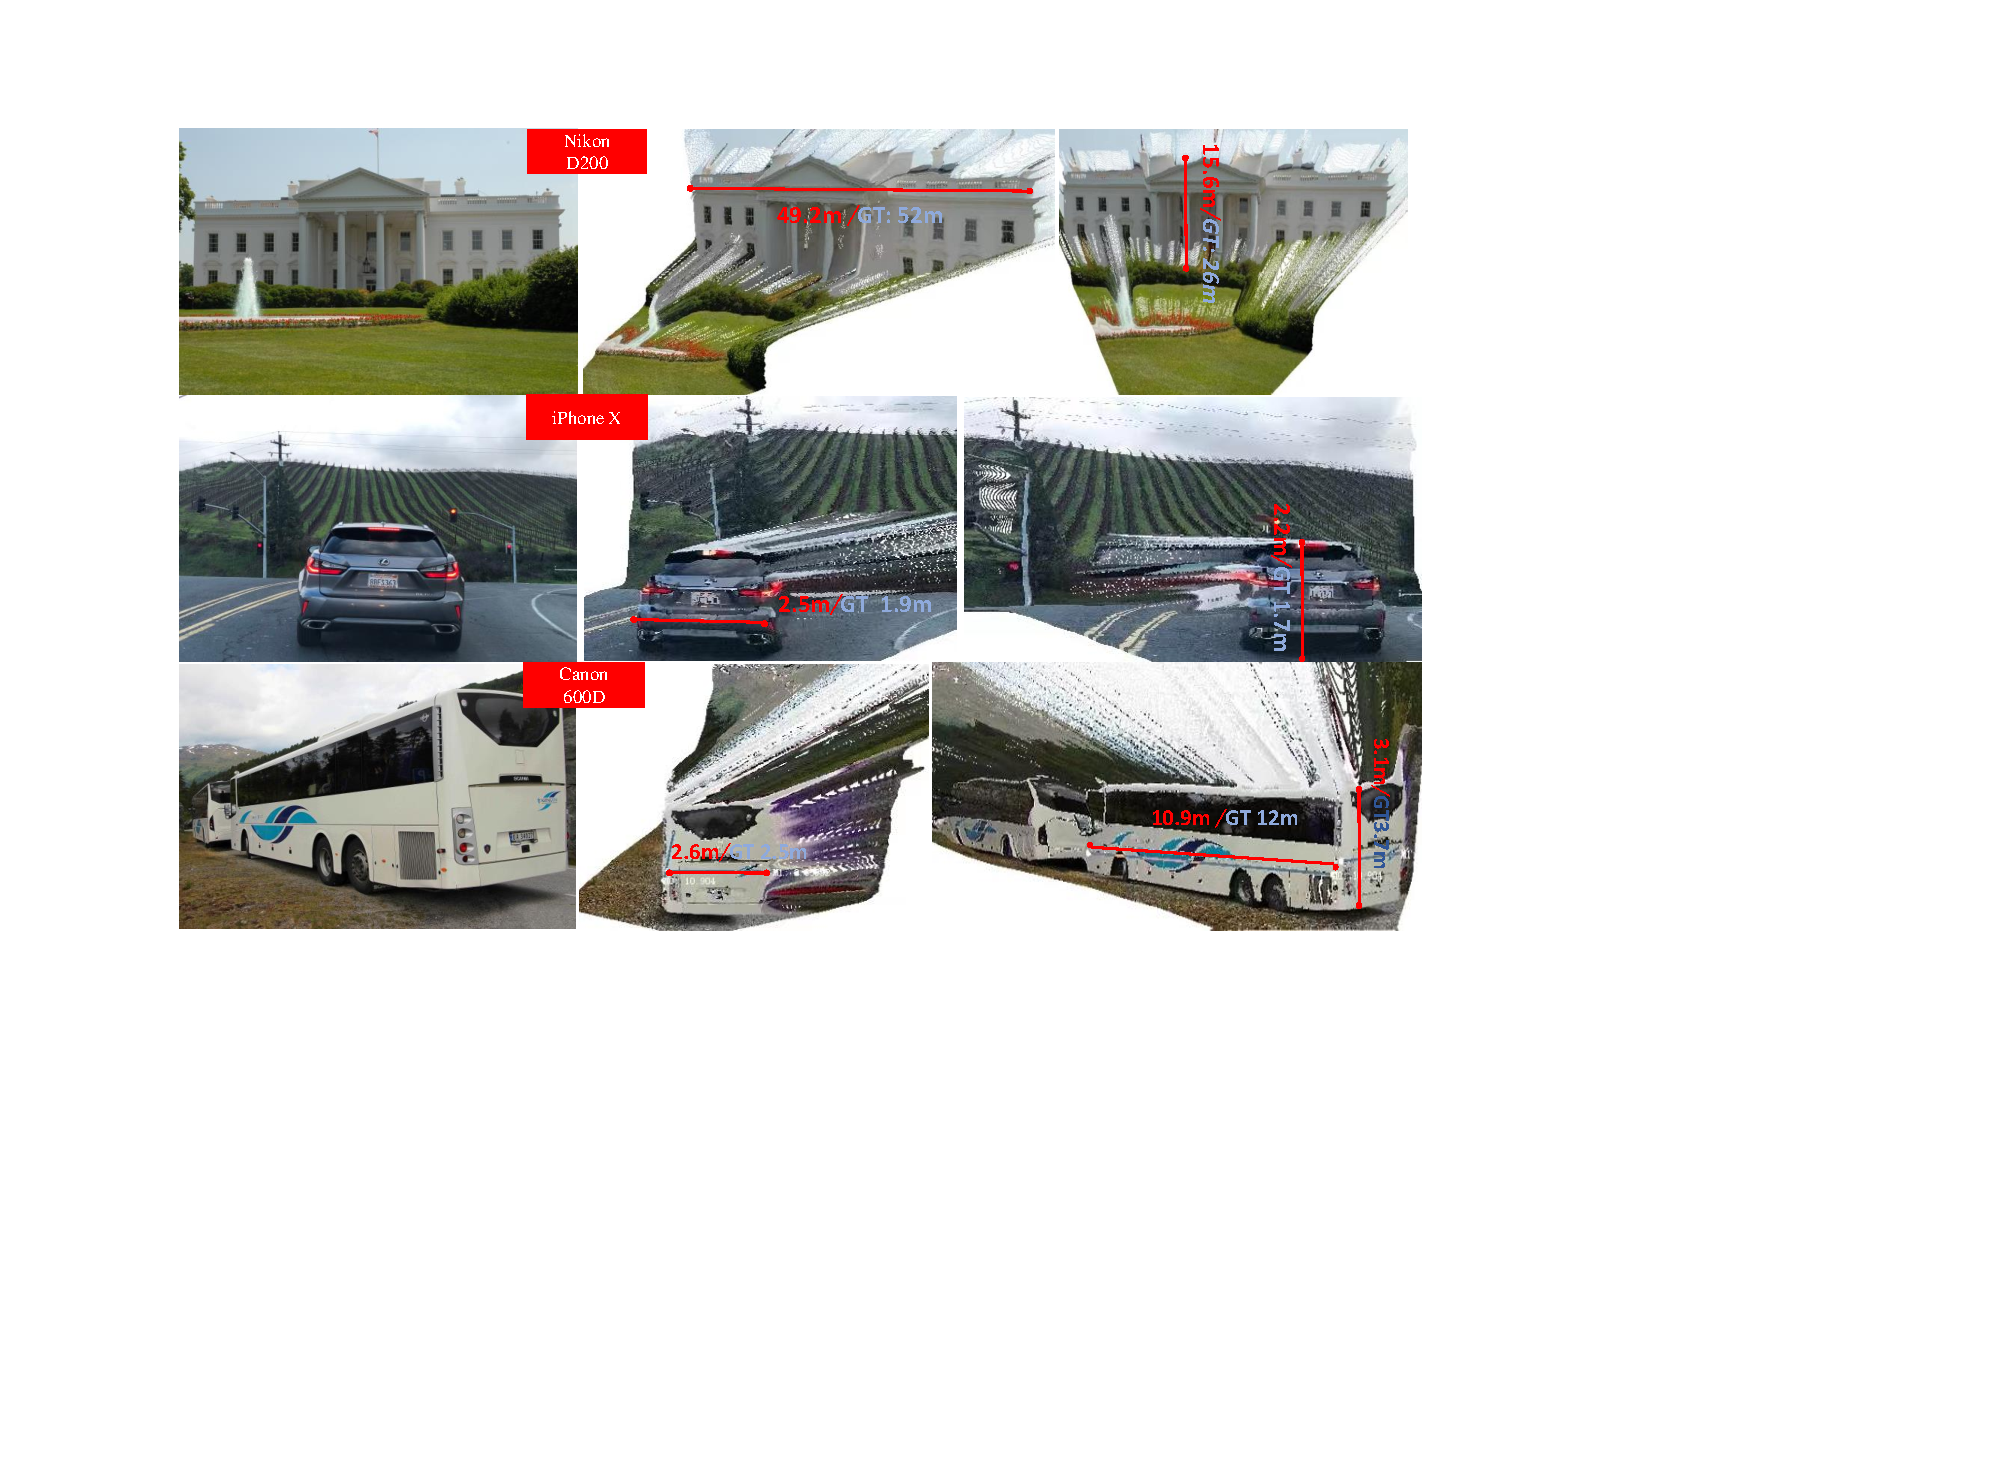
\includegraphics[width=0.5\textwidth]{./files/metrology_in_the_wild.pdf}
\vspace{-2 em}
\caption{\textbf{Reconstruction of in-the-wild scenes.} We collect several Flickr photos, which are captured by various cameras. With photos' metadata, we reconstruct the 3D metric shape and measure structures' sizes. Red and blue marks are ours and ground-truth sizes respectively. }
\label{fig: reconstruction in the wild.}
\vspace{-1em}
\end{figure}


\subsection{Applications Based on Our Method}
In these experiments, we apply the CSTM\_image model to various tasks. 

\noindent\textbf{3D scene reconstruction .}
To demonstrate our work can recover the 3D metric shape in the wild, we first do the quantitative comparison on 9 NYUv2 scenes, which are unseen during training. We predict the per-frame metric depth and then fuse them together with provided camera poses. Results are reported in Tab. \ref{tab: NYUD reconstruction cmp.}. We compare with the video consistent depth prediction method (RCVD~\cite{kopf2021rcvd}), the unsupervised video depth estimation method (SC-DepthV2~\cite{bian2021tpami}), the 3D scene shape recovery method (LeReS~\cite{leres}), affine-invariant depth estimation method (DPT~\cite{ranftl2021vision}), and the multi-view stereo reconstruction method (DPSNet~\cite{im2019dpsnet}). Apart from DPSNet and our method, other methods have to align the scale with the ground truth depth for each frame. Although our method does not aim for the video or multi-view reconstruction problem, our method can achieve promising consistency between frames and reconstruct much more accurate 3D scenes than others on these zero-shot scenes.  From the qualitative comparison in Fig.~\ref{fig: visual nyud reconstruction cmp.}. our reconstructions have much less noise and outliers. 

\noindent\textbf{Dense-SLAM mapping.}
Monocular SLAM is an important robotics application. It only relies on a monocular video input to create the trajectory and dense 3D mapping. Owing to limited photometric and geometric constraints, existing methods face serious scale drift problems in large scenes and cannot recover the metric information. Our robust metric depth estimation method is a strong depth prior to the SLAM system. To demonstrate this benefit,  we naively input our metric depth to the SOTA SLAM system, Droid-SLAM~\cite{teed2021droid}, and evaluate the trajectory on KITTI. We do not do any tuning on the original system. Trajectory comparisons are reported in Tab. \ref{tab: KITTI SLAM.}. As Droid-SLAM can access accurate per-frame metric depth, like an RGB-D SLAM, the translation drift ($t_{rel}$) decreases significantly. Furthermore, with our depths, Droid-SLAM can perform denser and more accurate 3D mapping. An example is shown in Fig.~\ref{Fig: first page fig.} and more cases are shown in the supplementary materials.   

We also test on the ETH3D SLAM benchmarks. Results are reported in Tab.~\ref{Tab: ETH3D SLAM}. Droid with our depths has much better SLAM performance. As the ETH3D scenes are all small-scale indoor scenes, the performance improvement is less than that on KITTI. 

\begin{table}[]
\renewcommand\arraystretch{1.1}
\caption{Comparison with SOTA SLAM methods on KITTI. We input predicted metric depth to the Droid-SLAM~\cite{teed2021droid} (`Droid+Ours'), which outperforms others by a large margin on trajectory accuracy.}
\centering
\resizebox{.98\linewidth}{!}{%
  \centering
  \small 
  \setlength{\tabcolsep}{0.5mm}{\begin{tabular}{@{} l |c|c|c|c|c|c|c@{}}
    \toprule
    \multirow{2}{*}{Method} & Seq 00 & Seq 02 & Seq 05 & Seq 06 & Seq 08 & Seq 09 & Seq 10 \\ \cline{2-8} 
      & \multicolumn{7}{c}{Translational RMS drift ($t_{rel}, \downarrow$) / Rotational RMS drift ($r_{rel}, \downarrow$)} \\ \hline
    GeoNet~\cite{yin2018geonet} & 27.6/5.72 & 42.24/6.14 & 
             20.12/7.67 & 
             9.28/4.34 & 
             18.59/7.85 & 
             23.94/9.81 & 
             20.73/9.1  \\
    VISO2-M~\cite{song2015high}  & 12.66/2.73 & 
             9.47/1.19 & 
             15.1/3.65 & 
             6.8/1.93 & 
             14.82/2.52 & 
             3.69/1.25 & 
             21.01/3.26  \\

    ORB-V2~\cite{murORB2} & 11.43/0.58 & 
             10.34/0.26 &
             9.04/0.26 & 
             14.56/0.26 & 
             11.46/0.28 & 
             9.3/0.26 & 
             2.57/0.32    \\
              
    Droid~\cite{teed2021droid} & 33.9/\textbf{0.29} & 
             34.88/\textbf{0.27} & 
             23.4/0.27 & 
             17.2/0.26 & 
             39.6/0.31 & 
             21.7/0.23 & 
             7/0.25   \\  \hline
             
    Droid+Ours & \textbf{1.44}/0.37 & 
             \textbf{2.64}/0.29 & 
             \textbf{1.44}/\textbf{0.25} & 
             \textbf{0.6}/\textbf{0.2} & 
             \textbf{2.2}/\textbf{0.3} & 
             \textbf{1.63}/\textbf{0.22} & 
             \textbf{2.73}/\textbf{0.23}    \\

    \bottomrule
  \end{tabular}}}
  \label{tab: KITTI SLAM.}
\end{table}

\begin{table}[t]
\caption{
Comparison of VO error on ETH3D benchmark. Droid SLAM system is input with our depth (`Droid + Ours'), and ground-truth depth (`Droid + GT'). The average trajectory error is reported.
}
 \resizebox{\linewidth}{!}{%
\begin{tabular}{l|llllll}
\hline
             & Einstein\_global & Manquin4 & Motion1 & Plantscene3 & sfm\_house\_loop & sfm\_lab\_room2 \\ \hline
& \multicolumn{6}{c}{Average trajectory error ($\downarrow$)}  \\ \hline
Droid        & 4.7                               & 0.88     & 0.83    & 0.78        & 5.64             & 0.55            \\ 
%Droid+LeReS  & 7.8                               & 0.91     & 0.95    & 0.80        & 6.9              & 0.55            \\ \hline
Droid + Ours & 1.5                               & 0.69     & 0.62    & 0.34        & 4.03             & 0.53            \\ 
Droid + GT   & 0.7                               & 0.006    & 0.024   & 0.006       & 0.96             & 0.013           \\ \hline
\end{tabular}}
\label{Tab: ETH3D SLAM}
\vspace{-1 em}
\end{table}

\noindent\textbf{Metrology in the wild.} To show the robustness and accuracy of our recovered metric 3D, we download Flickr photos captured by various cameras and collect coarse camera intrinsic parameters from their metadata. We use our CSTM\_image model to reconstruct their metric shape and measure structures' sizes (marked in red in Fig.~\ref{fig: reconstruction in the wild.}), while the ground-truth sizes are in blue. It shows that our measured sizes are very close to the ground-truth sizes. 






\subsection{Ablation Study}
\noindent\textbf{Ablation on canonical transformation.}
We study the effect of our proposed canonical transformation for the input images (`CSTM\_input') and the canonical transformation for the ground-truth labels (`CSTM\_output'). Results are reported in  Tab. \ref{table: importance of camera model.}. We train the model on sampled mixed data (55K images) and test it on 6 datasets. A naive baseline (`Ours w/o CSTM') is to remove CSTM modules and enforce the same supervision as ours. Without CSTM, the model is unable to converge when training on mixed metric datasets and cannot achieve metric prediction ability on zero-shot datasets. This is why recent mixed-data training methods compromise learning the affine-invariant depth to avoid metric issues. In contrast, our two CSTM methods both can enable the model to achieve the metric prediction ability, and they can achieve comparable performance. Tab. \ref{table:errors cmp on NYUD-V2} also shows comparable performance. Therefore, both adjusting the supervision and the input image appearance during training can solve the metric ambiguity issues. Furthermore, we compare with CamConvs~\cite{facil2019cam}, which encodes the camera model in the decoder with a 4-channel feature. `CamConvs' employ the same training schedule, model, and training data as ours. This method enforces the network to implicitly understand various camera models from the image appearance and then bridges the imaging size to the real-world size. We believe that this method challenges the data diversity and network capacity, thus their performance is worse than ours. 


\begin{table}[]
\caption{Effectiveness of our CSTM. CamConvs~\cite{facil2019cam} directly encodes various camera models in the network, while we perform a simple yet effective transformation to solve the metric ambiguity. Without CSTM, the model cannot achieve transferable metric prediction ability.}
\vspace{-1 em}
\scalebox{0.65}{
\begin{tabular}{l|lll|lll}
\toprule[1pt]
\multirow{2}{*}{Method}        & DDAD & Lyft & DS & NS & KITTI & NYU \\ 
        &\multicolumn{3}{c|}{Test set of train. data (AbsRel$\downarrow$)}     & \multicolumn{3}{c}{Zero-shot test set (AbsRel$\downarrow$)} \\  \hline 
w/o CSTM &$0.530$ &$0.582$  &$0.394$  &$1.00$ & $0.568$      &$0.584$  \\
CamConvs~\cite{facil2019cam}  &$0.295$ &$0.315$  &$0.213$ &$0.423$  &$0.178$      &$0.333$   \\
Ours CSTM\_image &$0.190$ &$0.235$  &$0.182$  &$0.197$ & $0.097$      &$0.210$ \\
Ours CSTM\_label &$0.183$ &$0.221$  &$0.201$  &$0.213$ & $0.081$      &$0.212$  \\
\toprule[1pt]
\end{tabular}}
\label{table: importance of camera model.}
\vspace{-1 em}
\end{table}





\noindent\textbf{Ablation on canonical space.}
We study the effect of the canonical camera here, \textit{i.e.}, the canonical focal length. We train the model on the small sampled dataset and test it on the validation set of training data and testing data. The average AbsRel error is calculated.  We experiment on 3 different focal lengths, \ie, 500, 1000, 1500. Experiments show that $focal=1000$ has slightly better performance than others, see Fig.~\ref{fig: canonical focal length.} for details. Thus we set the canonical focal length to 1000 in our experiments.

\begin{figure}[]
\centering
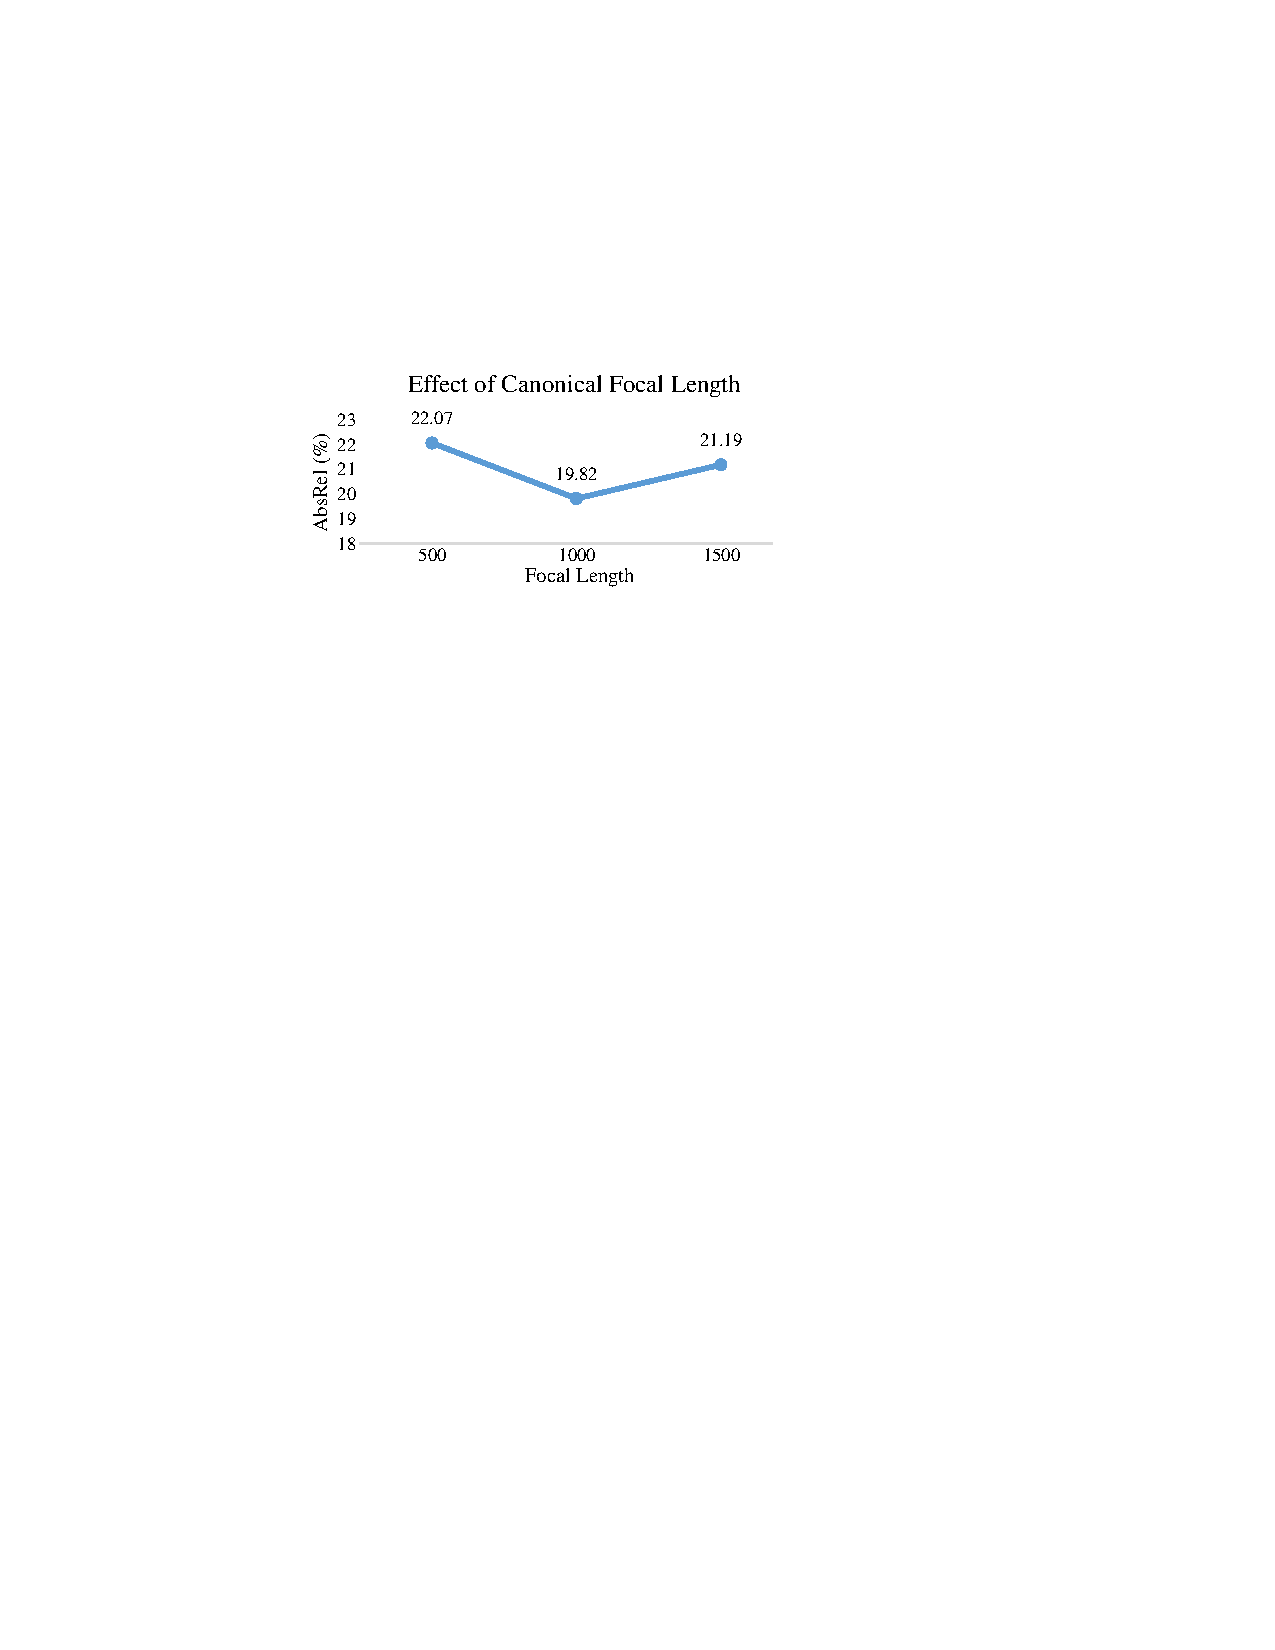
\includegraphics[width=0.3\textwidth]{./files/precision.pdf}
\caption{\textbf{Effect of different canonical focal lengths.} We experiment on different canonical focal lengths and find that too large or small focal lengths will impact the performance. }
\label{fig: canonical focal length.}
\end{figure}

\noindent\textbf{Effectiveness of 
the random proposal normalization loss.}
To show the effectiveness of our proposed random proposal normalization loss (RPNL), we experiment on the sampled small dataset. Results are shown in Tab.~\ref{table: effectiveness of rpnl.}. We test on the DDAD, Lyft, DrivingStereo (DS), NuScenes (NS), KITTI, and NYUv2.  The `baseline' employs all losses except our RPNL. We compare it with `baseline + RPNL' and `baseline + SSIL~\cite{Ranftl2020}'. We can observe that our proposed random proposal normalization loss can further improve the performance. 
In 
contrast, the scale-shift invariant loss~\cite{Ranftl2020}, which does the normalization on the whole image, can only slightly improve the performance. 
\begin{table}[]
\caption{Effectiveness of random proposal normalization loss. Baseline is supervised by `$L_{\PWN} + L_{\VNL} + L_{silog}$'. SSIL is the scale-shift invariant loss proposed in ~\cite{Ranftl2020}.}
\vspace{-1 em}
\scalebox{0.65}{
\begin{tabular}{l|lll|lll}
\toprule[1pt]
\multirow{2}{*}{Method}        & DDAD & Lyft & DS & NS & KITTI & NYUv2 \\ 
        &\multicolumn{3}{c|}{Test set of train. data (AbsRel$\downarrow$)}     & \multicolumn{3}{c}{Zero-shot test set (AbsRel$\downarrow$)} \\  \hline 
baseline  &$0.204$ &$0.251$  &$0.184$  &$0.207$ &$0.104$      &$0.230$     \\
baseline + SSIL~\cite{Ranftl2020} &$0.197$ &$0.263$  &$0.259$  &$0.206$ & $0.105$      &$0.216$     \\
baseline + RPNL   &$\textbf{0.190}$  &$\textbf{0.235}$  &$\textbf{0.182}$  &$\textbf{0.197}$ &$\textbf{0.097}$      &$\textbf{0.210}$     \\  \toprule[1pt]
\end{tabular}}
\label{table: effectiveness of rpnl.}
\vspace{-2 em}
\end{table}



\section{Conclusion} In this paper, we 
tackle 
the problem of reconstructing the 3D metric scene from a single monocular image. To solve the depth ambiguity in image appearance caused by various focal lengths, we propose a canonical camera space transformation method. With our method, we can easily merge millions of data captured by 10k cameras to train one metric depth model. To improve the robustness, we collected over $8$M data for training. Several zero-shot evaluations show the effectiveness and robustness of our work. We further show the ability to do metrology on randomly collected internet images and dense mapping on large-scale scenes. 

\section*{Acknowledgements}

This work was in part supported by National Key R\&D Program of China (No.\  2022ZD0118700).












\section{Appendix}
%  !TEX root = ../main.tex
~
% \vfill\eject
\section*{Appendix}
\setcounter{equation}{0}
\setcounter{subsection}{0}
\setcounter{section}{0}
\renewcommand{\theequation}{\arabic{equation}}
\renewcommand{\thesubsection}{\arabic{subsection}}
\renewcommand{\thesection}{\Alph{section}}

\section{Single-sideband Amplitude Modulation}\label{append:SSB}
In this section, we give mathematical proof that the baseband perturbation of SSB-AM signals can be recovered by commercial microphones. We initially compare the maximum energy of USB-AM and LSB-AM emitting the same perturbation when sound leakage occurs, and LSB-AM is 87\% of USB-AM. Thus, we adopt the USB-AM in our attacks due to its better inaudibility:
\begin{equation*}
\begin{aligned}
    & \text{USB-AM:}~ S_{USB}(t)=m{cos\omega_{c}t}-\hat{m}{sin\omega_{c}t}+cos\omega_{c}t\\
    & \text{LSB-AM:}~ S_{LSB}(t)=m{cos\omega_{c}t}+\hat{m}{sin\omega_{c}t}+cos\omega_{c}t
\end{aligned}
\label{equ:SSB_formula}
\end{equation*}
where the $\hat{m}$ is the conjugate of $m$. The microphone amplifier's output is below:
$$S_{out} = k_{1}S_{USB}(t) + k_{2}S_{USB}^2(t) + \cdots$$
The $S_{USB}^2(t)$ term has three components: a high-frequency $2\omega_{c}t$ components:
$$(m+1) \hat{m} \sin(2 \omega_c t)+\frac{m^2+2m+1-\hat{m}^2}{2} \cos(2\omega_c t)$$
a direct current (DC) term $\frac{1}{2}$ and an audible component $S_{aud}(t)=\frac{1}{2}(m^2+2m+\hat{m}^2)$.
$S_{USB}(t)$ and the high-frequency component are filtered by the low-pass filter because its frequency is above 25~kHz. The DC component is filtered by the microphone’s capacitor. Thus, the audible component $S_{aud}(t)$ that passes the microphone filtering system can function to ASR.
\vfill\eject

\section{Real-world Scenario}\label{append:attack_scenario}
Figure~\ref{fig:attack_actual} presents our real-world attack scenario.
\begin{figure}[h]
	\centering
	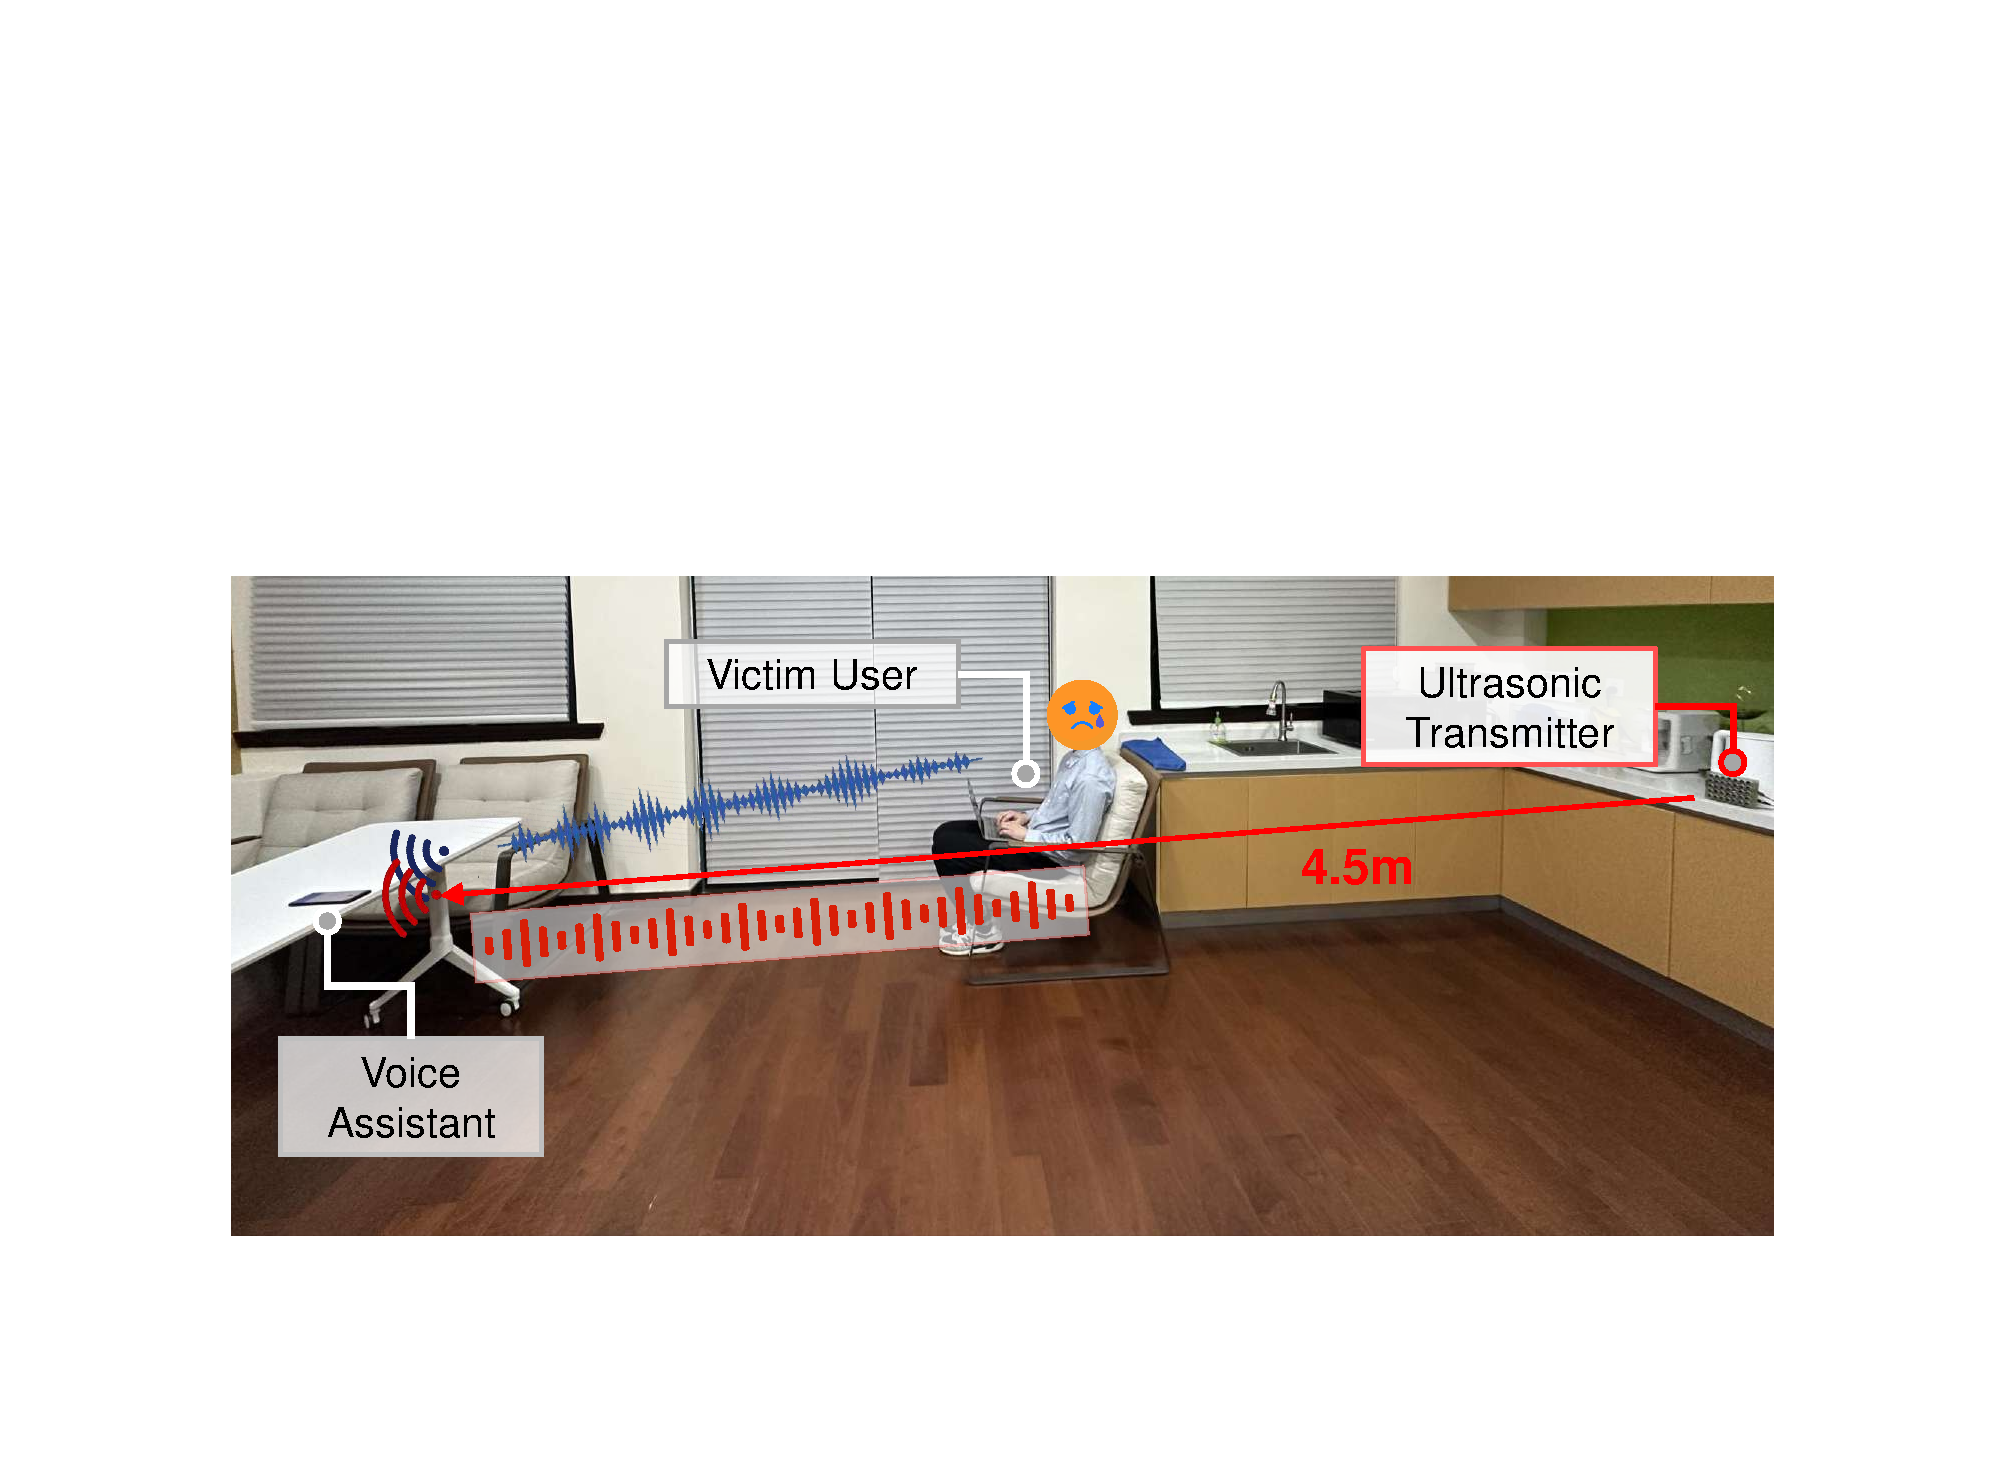
\includegraphics[width=0.48\textwidth]{exp_setup_actual2.pdf}
	\caption{\label{fig:attack_actual}Real-World Attack Scenario.}
	% \vspace{-10pt}
\end{figure}


\section{Algorithm of \alias}\label{append:algo1}
Given that technical workflow for the silence and universal perturbation are overall identical, the major differences are the optimization objective: $y_t/y_b$ and hyper-parameters. Therefore, we demonstrate \alias's representative optimization process of crafting a universal perturbation from scratch in Algorithm.~\ref{algo1}.
% \vfill\eject

\begin{algorithm}[h]
	\caption{Universal \alias Generation}
	\label{algo1}
	\LinesNumbered
	\KwIn{The ASR model with CTC Loss Computation module: $\mathcal{L}$, the maximum epoch: $\text{maxEpoch}$, the desired loss: $objValue$, with a scoring module: $S$, the learning rate: $\eta$, the preset time range: $T$.}
	\KwOut{The universal perturbation $\delta$}
	\textbf{Init} $\delta \gets 0^N$\\
	\For{$1$ to ${ maxEpoch}$}
	{
		${J} \gets 0$\\
            \For{$h_{\theta}\in U_H$, $n\in U_N$}
            {
                $\hat{e} = e^{-a_0 \omega_{c}^{n}d}$\\
                $\overline{\delta} = h_{\theta}\hat{e}\ast \overline{\delta:\hat{\xi}} + n$\\
                \For{$x\in U_x, g\in G, S_{(\cdot)}~{s.t.}~T$}
                {
                    $\Tilde{x}=\beta\cdot g\ast x$\\
                    $\Tilde{x_{\delta}} = clip(\Tilde{x}+\mathcal{S}_{(\overline{\delta})}, [-1,1])$\\
                    $J+=\mathcal{L}(\Tilde{x_{\delta}}, y_t)$
                }
            }
            Compute ${\nabla}_\mathcal{\delta}J$\\
            $\delta \gets \Omega_{Adam}(\delta+\eta\cdot {\nabla}_\mathcal{\delta}J )$\\
            $\delta \gets clip(\delta, [-1,1])$\\
            \If{$J \le objValue$}{break}
        }
	% return $\text{\alias}(\mathcal{A,K})$
	\normalsize
\end{algorithm}
\vfill\eject

\section{Targeted Commands Lists}\label{append:command_list}
Tab.\ref{tab:diff_commands} lists 10 different commands, corresponding to the performance of constructing target command-specific perturbations in experiment \textsection\ref{sec:eval_commands}.
\begin{table}[h]
	\centering
        \normalsize
		\caption{Attack with Different Targeted Commands}
		\renewcommand\arraystretch{0.9}
		\renewcommand\tabcolsep{1.5pt}
		\begin{threeparttable}
			\begin{tabular}{l|c|c}
                \toprule
                \textbf{Target Command} & \textbf{~~~~SR~~~~} & \textbf{~~CER~~} \\
				\midrule
                    ``Start recording''  & 100\% & 0\% \\ \midrule
				``Set a timer''  & 100\%  & 0\% \\ \midrule
				``Open the door''  & 100\% & 0\% \\ \midrule
				``Take the picture''  & 100\% & 0\% \\ \midrule
				``Call nine one one (911)''  & 100\% & 0\% \\ \midrule
				``Cancel my morning alarm''  & 100\% & 0\% \\ \midrule
                    ``Turn on airplane mode'' & 94.39\% & 0.28\% \\ \midrule
                    ``Open my photo album''  & 95.03\% & 0.50\% \\ \midrule
				``What is going on Twitter?''  & 100\% & 0\% \\ \midrule
                    ``Mute volume and turn off the WiFi'' & 92.82\% & 0.21\% \\
				\bottomrule
			\end{tabular}
		% \vspace{-10pt}
		\end{threeparttable}
		\label{tab:diff_commands}
\end{table}
% \vfill\eject


\section{Different Attack Angles}\label{append:eval_angles}
In this experiment, we keep the recording device's bottom microphone spatially within the ultrasound beam's coverage and set the attack distance to 2.5m. We rotate the recording device from 0\degree to 180\degree at 15\degree intervals, among which 90\degree means the ultrasound directly points to the bottom microphone. Under each angle, we play 40 benign commands and emit the universal IAP.
Eventually, we collected 520 mixed audio signals from 13 angles. As shown in Fig.~\ref{fig:attack_angle}, although ultrasound is highly directional, we find that there is no significant difference with 100\% success rate among different angles within 15\degree$\sim$150\degree. As the deployed location of bottom microphones varies with different phones, therefore attack performance is not symmetrical with angles (i.e., 79\% at 0\degree and 49\% at 180\degree). Overall, as most voice-interface devices nowadays are equipped with omnidirectional microphones, \alias can be effective as long as the beam can cover the bottom microphone. 
\begin{figure}[h]
    \centering
    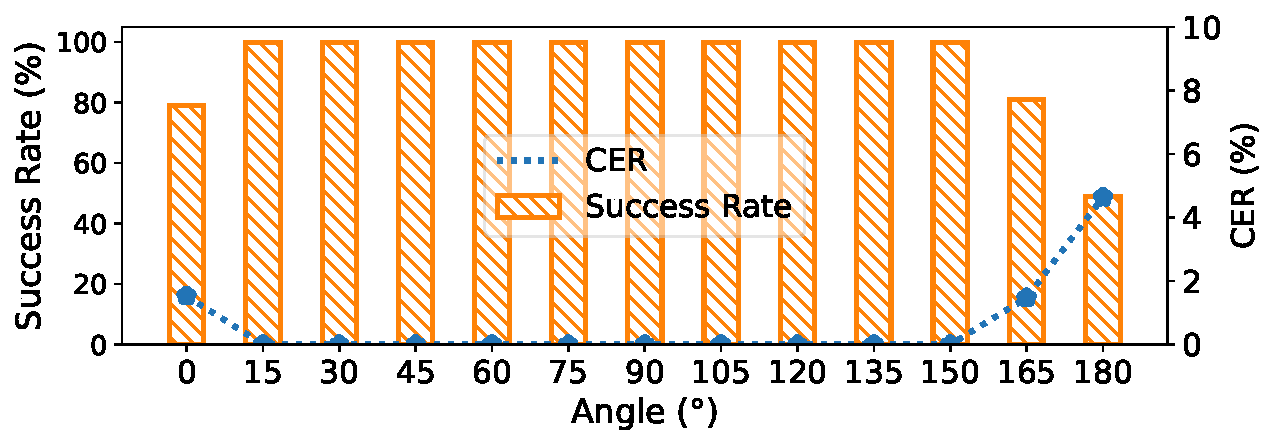
\includegraphics[width=0.45\textwidth]{attack_angle.pdf}
    % \vspace{-10pt}
    \caption{\alias's performance at different angles.}
    \label{fig:attack_angle}
\end{figure}

% \vfill\eject

\section{Different Speech \& Perturbation Loudness}\label{append:loudness_compare}
Fig.~\ref{fig:loudness_compare} shows the success rate and CER of our experiments on the relative energies between the attack perturbation and speech.
\begin{figure}[h]
	% \vspace{-7pt}
	\centering  %居中
		\subfigure[Success Rate (\%)]{   %第一张子图
		\begin{minipage}[t]{0.22\textwidth}
			\centering
                % \hspace{-0.25\linewidth}
			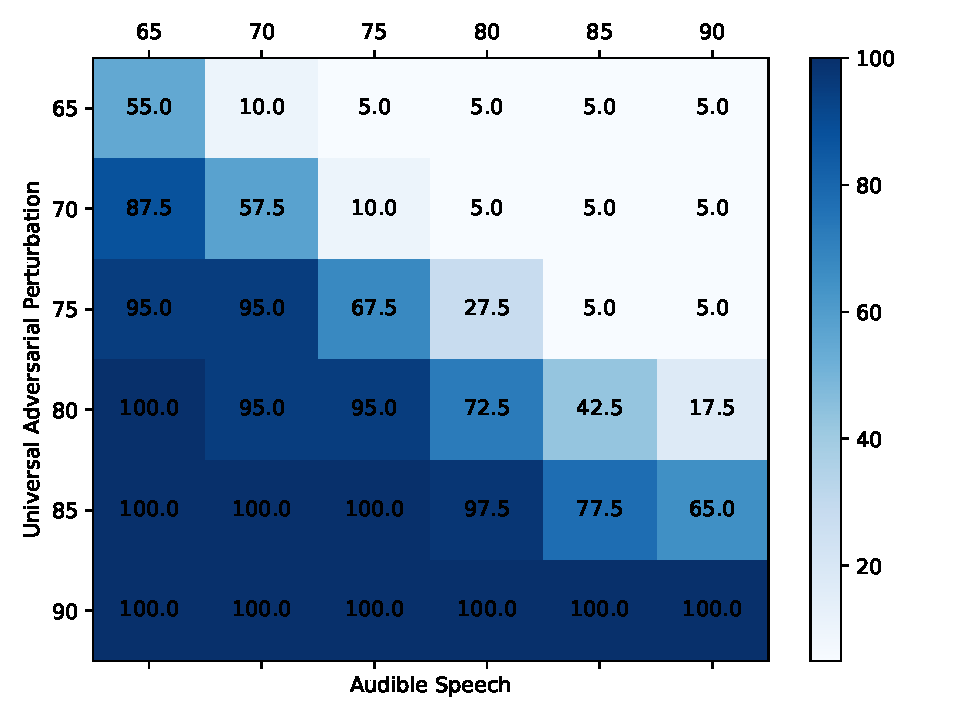
\includegraphics[width=1.1\textwidth]{snr_SR.pdf} % height=0.765\linewidth
		\end{minipage}
		}
	\subfigure[CER (\%)]{   %第一张子图
	\begin{minipage}[t]{0.22\textwidth}
		\centering
            % \hspace{-0.25\linewidth}
		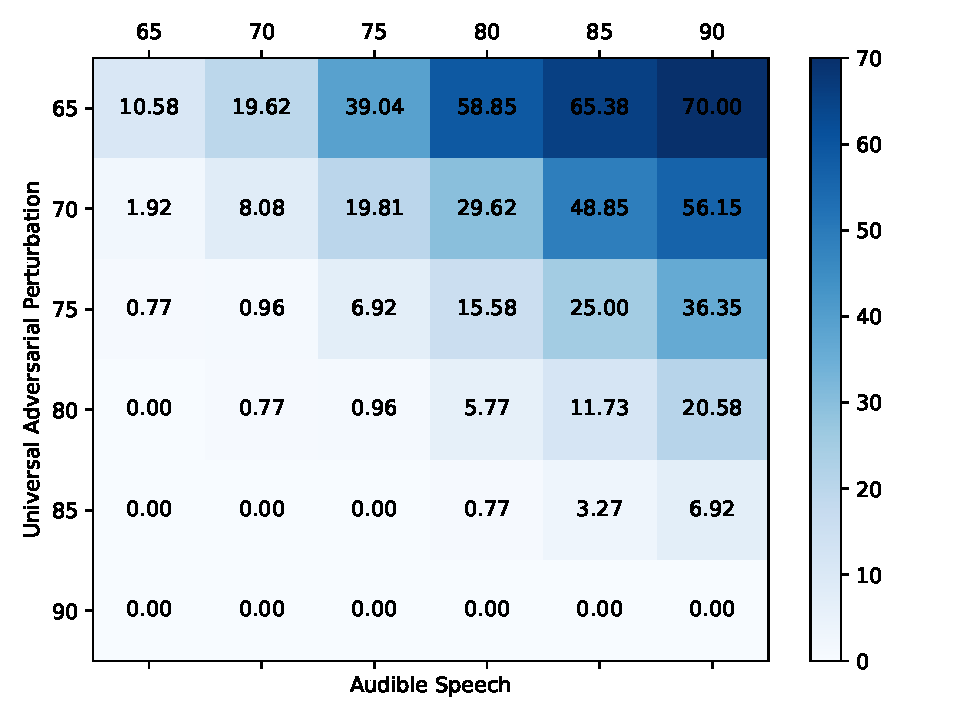
\includegraphics[width=1.1\textwidth]{snr_CER.pdf} 
	\end{minipage}
	}
	% \vspace{-10pt}
	\caption{The performance of loudness relationship between user speech and perturbation.}    %大图名称
	\label{fig:loudness_compare}    %图片引用标记
	% \vspace{-5pt}
\end{figure}
% \vfill\eject

\section{User Testing}\label{append:user_test}
In this section, we elaborate on the \textit{Man-in-the-middle} attack strategy, whose effect is akin to experiencing network congestion when users use the ASR service, resulting in slower responses. Prolonged latency can make users feel uncomfortable while using the service. 
To assess user awareness under such delays, we design 10 scenarios, each consisting of an audio clip that simulates a user issuing a command to the ASR system with random delays (1-5 seconds) before the voice assistant executes the command. 
We collected test results from 140 college students of different majors. As shown in Figure~\ref{fig:user_latency}, when the delay time is less than 2.7 seconds (the junction point of two distribution curves), more users find the ASR service comforting than uncomfortable. 
The participants are also asked to fill in what they think the cause is if they experience an uncomfortable delay when using the ASR service.
Only 11 out of 140 participants suspect an attack, while almost all others attribute the delay to network latency/congestion or device stuck, suggesting that this strategy poses a hidden attack.
We believe that users' suspicion may also be related to their disciplinary background, e.g., users with knowledge of cybersecurity are more likely to consider the possibility of an attack.

\begin{figure}[h]
    \centering
    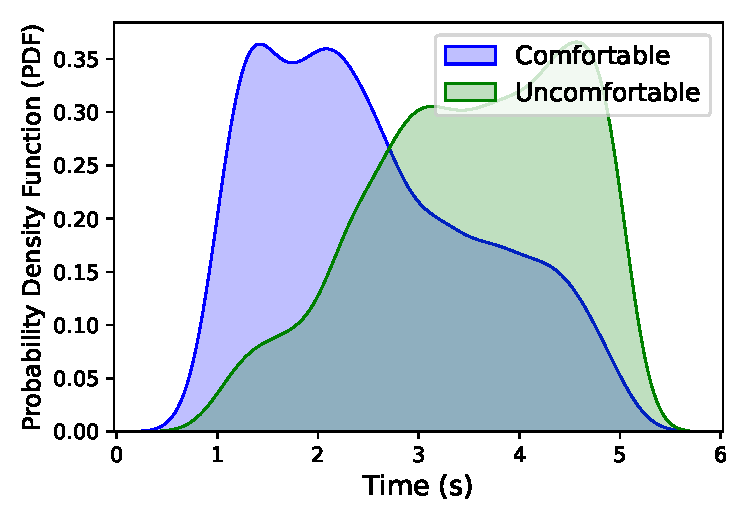
\includegraphics[width=0.45\textwidth]{latency.pdf}
    \caption{The probability distribution of users' awareness during a \textit{man-in-the-middle} attack under different delay conditions (similar to network latency). ``Comfortable'': the situation where users find the ASR service is normal and are not aware of the attack; ``Uncomfortable'': the delay may cause them to feel uncomfortable or unusual.}
    \label{fig:user_latency}
\end{figure}






{\small
\bibliographystyle{./ICCV2023/ieee_fullname}
\bibliography{./ICCV2023/egbib}
}

\end{document}